% !TeX program = xelatex
% !TeX encoding = UTF-8
\documentclass[12pt,openany,oneside]{book}

\usepackage[a4paper,top=23mm,bottom=25mm,left=25mm,right=25mm,headheight=17pt]{geometry}
\usepackage{amsmath,amssymb,amsfonts,mathtools,bm}
\usepackage{amsthm}
\usepackage{booktabs,longtable,array,multirow,tabularx}
\usepackage{graphicx}
\graphicspath{{figures/}}
\usepackage{xcolor}
\usepackage{tikz}
\usetikzlibrary{arrows.meta,positioning,calc,fit,shapes.geometric,decorations.pathreplacing,matrix,patterns,3d}
\usepackage[most]{tcolorbox}
\usepackage{enumitem}
\usepackage{listings}
\usepackage{caption}
\usepackage{subcaption}
\usepackage{float}
\usepackage{fancyhdr}
\usepackage{titlesec}
\usepackage{setspace}
\usepackage{microtype}
\usepackage{hyperref}
\usepackage{xepersian}

\IfFontExistsTF{Amiri}
  {\settextfont[Scale=1.08]{Amiri}\setdigitfont{Amiri}}
  {\settextfont[Scale=1.05]{Noto Naskh Arabic}\setdigitfont{Noto Naskh Arabic}}
\IfFontExistsTF{DejaVu Serif}
  {\setlatintextfont{DejaVu Serif}}
  {\setlatintextfont{Latin Modern Roman}}
\IfFontExistsTF{DejaVu Sans Mono}
  {\setmonofont{DejaVu Sans Mono}}
  {\setmonofont{Latin Modern Mono}}

\definecolor{DeepBlue}{HTML}{163A5F}
\definecolor{Accent}{HTML}{B34B35}
\definecolor{SoftBlue}{HTML}{EAF2F8}
\definecolor{SoftGold}{HTML}{FFF6DF}
\definecolor{SoftGreen}{HTML}{EAF7EF}
\definecolor{SoftRed}{HTML}{FCEDEC}
\definecolor{SoftGray}{HTML}{F4F5F6}
\definecolor{CodeGray}{HTML}{F7F7F7}

\hypersetup{
  colorlinks=true,
  linkcolor=DeepBlue,
  citecolor=Accent,
  urlcolor=Accent,
  pdftitle={پردازش تصویر در دهه آینده ـ فصل نهم: ویژگی، تطبیق و بازشناسی کلاسیک},
  pdfauthor={جزوه درس کارشناسی ارشد}
}

\setstretch{1.22}
\setlength{\parskip}{0.35em}
\setlength{\parindent}{1.3em}
\setlist[itemize]{itemsep=0.25em,topsep=0.35em,leftmargin=9mm}
\setlist[enumerate]{itemsep=0.25em,topsep=0.35em,leftmargin=10mm}

\pagestyle{fancy}
\fancyhf{}
\fancyhead[R]{\small\thepage}
\fancyhead[L]{\small\nouppercase{\leftmark}}
\renewcommand{\headrulewidth}{0.4pt}

\titleformat{\chapter}[display]
  {\normalfont\huge\bfseries\color{DeepBlue}}
  {\filleft\Large فصل \thechapter}
  {8pt}
  {\filright}
\titleformat{\section}{\Large\bfseries\color{DeepBlue}}{\thesection}{0.7em}{}
\titleformat{\subsection}{\large\bfseries\color{Accent}}{\thesubsection}{0.7em}{}
\titleformat{\subsubsection}{\normalsize\bfseries\color{DeepBlue}}{\thesubsubsection}{0.7em}{}

\newtheorem{definition}{تعریف}[chapter]
\newtheorem{theorem}{قضیه}[chapter]
\newtheorem{proposition}{گزاره}[chapter]
\newtheorem{lemma}{لم}[chapter]
\newtheorem{example}{مثال}[chapter]
\newtheorem{remark}{نکته}[chapter]
\newtheorem{corollary}{نتیجه}[chapter]
\renewcommand{\proofname}{اثبات}

\newtcolorbox{learningbox}{colback=SoftBlue,colframe=DeepBlue,title=اهداف یادگیری,fonttitle=\bfseries,breakable,enhanced}
\newtcolorbox{keybox}[1][]{colback=SoftGold,colframe=Accent,title={#1},fonttitle=\bfseries,breakable,enhanced}
\newtcolorbox{futurebox}{colback=SoftGreen,colframe=green!50!black,title=پل به دهه آینده,fonttitle=\bfseries,breakable,enhanced}
\newtcolorbox{warningbox}{colback=SoftRed,colframe=red!65!black,title=خطای رایج,fonttitle=\bfseries,breakable,enhanced}
\newtcolorbox{workshopbox}[1][]{colback=SoftGray,colframe=black!55,title={کارگاه کد و آزمایش: #1},fonttitle=\bfseries,breakable,enhanced}
\newtcolorbox{researchbox}[1][]{colback=white,colframe=purple!65!black,title={خواندن مقاله و استاندارد: #1},fonttitle=\bfseries,breakable,enhanced}
\newtcolorbox{videobox}{colback=white,colframe=DeepBlue,title=تقسیم پیشنهادی ویدئوهای ۱۵ دقیقه‌ای,fonttitle=\bfseries,breakable,enhanced}
\newtcolorbox{proofbox}[1][]{colback=white,colframe=DeepBlue!65,title={مسیر اثبات: #1},fonttitle=\bfseries,breakable,enhanced}
\newtcolorbox{codecontract}{colback=SoftBlue,colframe=Accent,title=قرارداد میان ریاضیات و کد,fonttitle=\bfseries,breakable,enhanced}
\newtcolorbox{summarybox}{colback=SoftBlue,colframe=DeepBlue,title=جمع‌بندی فصل,fonttitle=\bfseries,breakable,enhanced}
\newtcolorbox{goalbox}{colback=SoftBlue,colframe=DeepBlue,title=هدف فصل,fonttitle=\bfseries,breakable,enhanced}
\newtcolorbox{principlebox}{colback=SoftGold,colframe=Accent,title=اصل راهنما,fonttitle=\bfseries,breakable,enhanced}
\newtcolorbox{algorithmbox}[1]{colback=SoftGray,colframe=DeepBlue,title={#1},fonttitle=\bfseries,breakable,enhanced}
\newtcolorbox{theorembox}[1]{colback=white,colframe=purple!65!black,title={#1},fonttitle=\bfseries,breakable,enhanced}
\newtcolorbox{applicationbox}[1][]{colback=SoftGreen,colframe=green!45!black,title={کاربرد مهندسی: #1},fonttitle=\bfseries,breakable,enhanced}

\newcommand{\R}{\mathbb{R}}
\newcommand{\C}{\mathbb{C}}
\newcommand{\N}{\mathbb{N}}
\newcommand{\Z}{\mathbb{Z}}
\newcommand{\E}{\mathbb{E}}
\newcommand{\Var}{\operatorname{Var}}
\newcommand{\Cov}{\operatorname{Cov}}
\newcommand{\Prob}{\mathbb{P}}
\newcommand{\norm}[1]{\left\lVert #1\right\rVert}
\newcommand{\abs}[1]{\left\lvert #1\right\rvert}
\newcommand{\inner}[2]{\left\langle #1,#2\right\rangle}
\newcommand{\trans}{^{\mathsf T}}
\newcommand{\herm}{^{\mathsf H}}
\newcommand{\inv}{^{-1}}
\newcommand{\vect}[1]{\bm{#1}}
\newcommand{\mat}[1]{\bm{#1}}
\newcommand{\argmin}{\operatorname*{arg\,min}}
\newcommand{\argmax}{\operatorname*{arg\,max}}
\newcommand{\trace}{\operatorname{tr}}
\newcommand{\diag}{\operatorname{diag}}
\newcommand{\rank}{\operatorname{rank}}
\newcommand{\sign}{\operatorname{sign}}
\newcommand{\softmax}{\operatorname{softmax}}
\newcommand{\dist}{\operatorname{dist}}
\newcommand{\supp}{\operatorname{supp}}
\newcommand{\NCC}{\operatorname{NCC}}
\newcommand{\IoU}{\operatorname{IoU}}
\newcommand{\AP}{\operatorname{AP}}
\newcommand{\mAP}{\operatorname{mAP}}
\newcommand{\Hamm}{d_{\mathrm H}}
\newcommand{\SE}{\mathrm{SE}}
\newcommand{\SO}{\mathrm{SO}}

\lstset{
  language=Python,
  basicstyle=\small\ttfamily\color{black},
  columns=fullflexible,
  keepspaces=true,
  backgroundcolor=\color{CodeGray},
  frame=single,
  rulecolor=\color{black!25},
  numbers=left,
  numberstyle=\tiny,
  breaklines=true,
  showstringspaces=false,
  keywordstyle=\bfseries\color{DeepBlue},
  commentstyle=\itshape\color{black!65},
  stringstyle=\color{Accent},
  tabsize=4
}

\begin{document}

\begin{titlepage}
\centering
\vspace*{0.9cm}
{\color{DeepBlue}\rule{0.9\textwidth}{1.1pt}}\\[1.0cm]
{\Huge\bfseries پردازش تصویر در دهه آینده\\[0.3cm]}
{\LARGE\bfseries از عمق ریاضیات تا مهندس حرفه‌ای\\[0.85cm]}
{\Large کتاب ـ جزوه درس کارشناسی ارشد و آزمایشگاه پژوهش‌محور\\[1.1cm]}

\begin{tikzpicture}[node distance=8mm]
\node[draw=DeepBlue,very thick,rounded corners=3mm,fill=SoftBlue,
      minimum width=13.1cm,minimum height=4.8cm,text width=12.6cm,align=center] (a)
{\Large\bfseries فصل نهم\\[2mm]
\large ویژگی، تطبیق و بازشناسی کلاسیک\\[1mm]
\normalsize از تطبیق قالب، گوشه و فضای مقیاس تا SIFT و ORB،
راستی‌آزمایی مقاوم، کلمات بصری، HOG--SVM و گذار به تطبیق آموختنی};
\node[below=7mm of a,align=center,text width=12.8cm] {
تصویر هنگامی به حافظه، نقشه، شیء یا کلاس متصل می‌شود که از آن نمایش قابل تکرار، قابل تطبیق و قابل تصمیم استخراج کنیم.
این فصل هندسه، آمار و الگوریتم را در یک خط لوله مشترک گرد می‌آورد.};
\end{tikzpicture}

\vfill
{\large نسخه تفصیلی درس ـ تابستان ۱۴۰۵ / ۲۰۲۶}\\[0.4cm]
{\normalsize قابل کامپایل با \lr{TeX Live + TeXstudio + XeLaTeX}}\\[0.8cm]
{\color{DeepBlue}\rule{0.9\textwidth}{1.1pt}}
\end{titlepage}

\frontmatter

\chapter*{یادداشت روش‌شناختی فصل نهم}
\addcontentsline{toc}{chapter}{یادداشت روش‌شناختی فصل نهم}
در فصل‌های پیشین آموختیم تصویر چگونه تشکیل، نویزی، بازسازی و قطعه‌بندی می‌شود. اکنون پرسش عوض می‌شود:
کدام بخش تصویر ارزش به‌یادسپاری دارد، چگونه همان ساختار را زیر تغییر نور، چرخش، مقیاس و دیدگاه دوباره پیدا کنیم، و چگونه
از مجموعه این تطابق‌ها برای بازشناسی شیء یا صحنه استفاده کنیم؟ پاسخ تاریخی بینایی ماشین، خط لوله‌ای چندمرحله‌ای است:
\[
\text{آشکارسازی}\longrightarrow\text{توصیف}\longrightarrow\text{تطبیق}
\longrightarrow\text{راستی‌آزمایی هندسی}\longrightarrow\text{بازشناسی}.
\]
هر مرحله فرضی را به مرحله بعد تحویل می‌دهد. اگر آشکارساز تکرارپذیر نباشد، بهترین توصیفگر نیز شکست می‌خورد؛ اگر
توصیفگر متمایز نباشد، نزدیک‌ترین همسایه پر از تطابق کاذب است؛ اگر هندسه آزموده نشود، شباهت بافتی به‌اشتباه به
وجود یک شیء تعبیر می‌شود؛ و اگر تجمیع ویژگی‌ها هندسه و فراوانی را نابود کند، بازشناسی ضعیف خواهد شد.

\begin{goalbox}
هدف فصل حفظ چهار کمیت در تمام بحث‌هاست:
\begin{enumerate}
\item \textbf{هم‌وردایی و ناوردایی:} ویژگی زیر تبدیل تصویر چگونه جابه‌جا یا ثابت می‌ماند؟
\item \textbf{تکرارپذیری و دقت مکانی:} آیا همان ساختار دوباره یافت می‌شود و مکان آن چقدر خطا دارد؟
\item \textbf{تمایزبخشی و احتمال ابهام:} یک توصیفگر چند وصله نامرتبط را مشابه می‌بیند؟
\item \textbf{هزینه و مقیاس‌پذیری:} استخراج، جست‌وجو و راستی‌آزمایی برای هزار تصویر یا یک میلیارد ویژگی چقدر هزینه دارد؟
\end{enumerate}
\end{goalbox}

\begin{figure}[H]
\centering
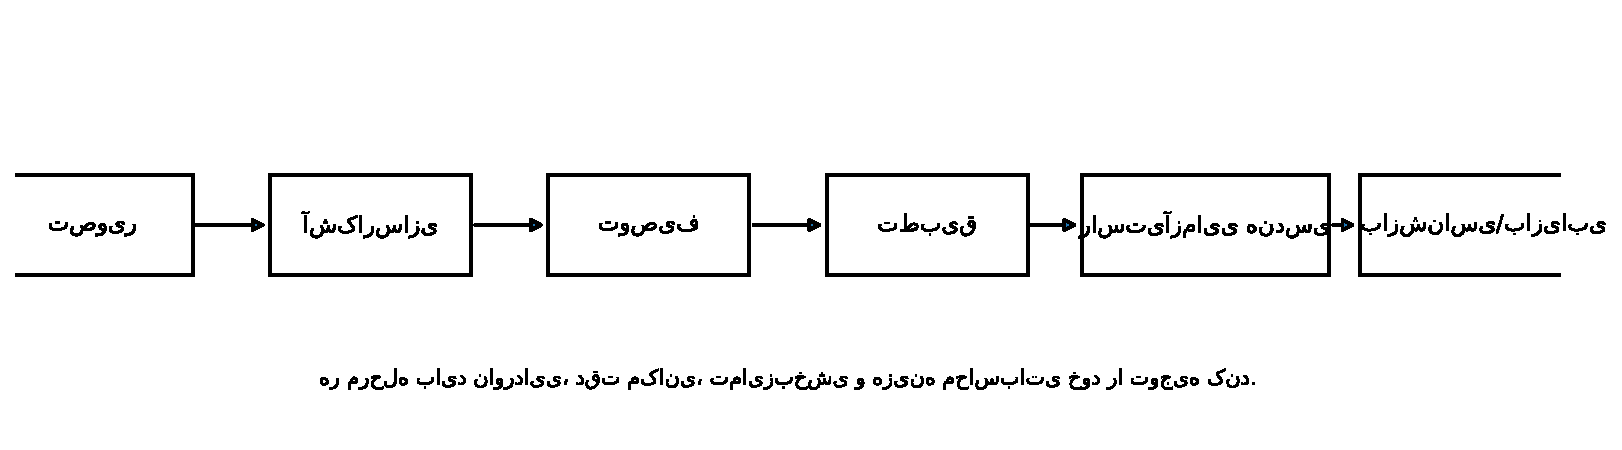
\includegraphics[width=0.97\textwidth]{fig09_01_pipeline.pdf}
\caption{خط لوله کلاسیک ویژگی تا بازشناسی. روش‌های جدید بخشی از این بلوک‌ها را می‌آموزند یا ادغام می‌کنند، اما پرسش‌های بنیادی آن‌ها پابرجاست.}
\label{fig:pipeline}
\end{figure}

\chapter*{نقشه فشرده فصل}
\addcontentsline{toc}{chapter}{نقشه فشرده فصل}
\begin{longtable}{p{35mm}p{104mm}}
\toprule
محور & پرسش و خروجی آموزشی \\
\midrule
مدل تبدیل & روشنایی، نویز، چرخش، مقیاس، آفین و پرسپکتیو چگونه بر وصله اثر می‌گذارند؟ \\
تطبیق قالب & SSD، SAD، NCC، ZNCC و phase correlation چه فرض‌هایی دارند و چگونه سریع می‌شوند؟ \\
نقطه کلیدی & Moravec، Harris، Shi--Tomasi، FAST و AGAST چه ساختاری را آشکار می‌کنند؟ \\
فضای مقیاس & Gaussian scale-space، LoG، DoG، Hessian و affine adaptation چگونه ناوردایی می‌سازند؟ \\
توصیفگر & SIFT، RootSIFT، HOG، shape context و توصیفگرهای دودویی چه اطلاعاتی را نگه می‌دارند؟ \\
تطبیق & فاصله اقلیدسی، کسینوسی، ماهالانوبیس و همینگ؛ ratio test، cross-check و assignment چگونه انتخاب می‌شوند؟ \\
راستی‌آزمایی & RANSAC، PROSAC، LO-RANSAC و MAGSAC++ چگونه مدل هندسی را از برون‌ریزها جدا می‌کنند؟ \\
بازشناسی مستقیم & template، generalized Hough، chamfer، PCA/LDA، kNN، SVM و boosting چه زمانی مناسب‌اند؟ \\
واژگان بصری & BoVW، TF--IDF، spatial pyramid، VLAD و Fisher Vector چگونه ویژگی‌های محلی را به بردار تصویر تبدیل می‌کنند؟ \\
ارزیابی & repeatability، matching score، pose AUC، mAP، confusion و آزمون تاب‌آوری چگونه گزارش می‌شوند؟ \\
مرز دانش & SuperPoint، LightGlue، LoFTR، RoMa، OmniGlue، RDD و تطبیق‌گرهای ۲۰۲۶ چه چیزی را تغییر داده‌اند؟ \\
مهندسی & چگونه خط لوله reproducible، سریع، بدون leakage و دارای failure taxonomy ساخته شود؟ \\
\bottomrule
\end{longtable}

\tableofcontents
\mainmatter
\setcounter{chapter}{8}
\chapter{ویژگی، تطبیق و بازشناسی کلاسیک}

\begin{learningbox}
در پایان فصل، دانشجو باید بتواند:
\begin{itemize}
\item پاسخ آشکارساز Harris، LoG/DoG و Hessian را از مدل تغییر وصله استخراج کند؛
\item مفهوم هم‌وردایی آشکارساز و ناوردایی توصیفگر را با زبان گروه تبدیل توضیح دهد؛
\item SIFT و HOG را نه به‌صورت نام، بلکه به‌صورت histogram جهت‌دار، نرمال‌سازی و pooling پیاده‌سازی کند؛
\item برای توصیفگرهای حقیقی و دودویی معیار فاصله و جست‌وجوی مناسب انتخاب کند؛
\item تعداد iteration لازم RANSAC را محاسبه و degeneracy و threshold را تحلیل کند؛
\item BoVW، spatial pyramid، VLAD و Fisher Vector را از descriptorهای محلی بسازد؛
\item HOG+SVM، Eigenfaces/Fisherfaces و AdaBoost cascade را آموزش و ارزیابی کند؛
\item روش کلاسیک را با SuperPoint/LightGlue/LoFTR در پروتکل هندسی عادلانه مقایسه کند؛
\item بین دقت تطبیق، پوشش، سرعت، حافظه، قابلیت توضیح و robustness تصمیم مهندسی بگیرد.
\end{itemize}
\end{learningbox}

\section{ویژگی چیست؟ از مقدار پیکسل تا ساختار قابل تطبیق}
فرض کنید تصویر مشاهده‌شده از یک صحنه مرجع با تبدیل هندسی $g$، تبدیل فوتومتریک $\phi$ و نویز $n$ ساخته شود:
\begin{equation}
I_2(\vect u)=\phi\!\left(I_1(g^{-1}\vect u)\right)+n(\vect u).
\label{eq:formation_feature}
\end{equation}
هدف ویژگی، ساخت نگاشتی $\Phi$ است که اطلاعات مورد نیاز وظیفه را حفظ و تغییرات مزاحم را حذف کند. دو مفهوم باید جدا شوند.

\begin{definition}[هم‌وردایی آشکارساز]
اگر آشکارساز $D$ مجموعه نواحی یا نقاط را برگرداند، نسبت به تبدیل $g$ هم‌ورداست هرگاه
\[
D(I\circ g^{-1})=gD(I).
\]
یعنی مکان ویژگی همراه تصویر تبدیل می‌شود، نه اینکه ثابت بماند.
\end{definition}

\begin{definition}[ناوردایی توصیفگر]
توصیفگر $\Psi$ نسبت به $g$ ناورداست اگر پس از نرمال‌سازی ناحیه
\[
\Psi(I,\vect p)\approx \Psi(I\circ g^{-1},g\vect p).
\]
برابری دقیق معمولاً ناممکن و حتی نامطلوب است؛ تقریب باید تغییرات مجاز را تحمل و تفاوت ساختارهای واقعاً متفاوت را حفظ کند.
\end{definition}

\begin{principlebox}
آشکارساز باید \textbf{کجا} را پایدار پیدا کند؛ توصیفگر باید بگوید \textbf{چه چیزی} در آنجاست؛ matcher باید شباهت را به
فرضیه correspondence تبدیل کند؛ و هندسه باید بررسی کند آیا مجموعه فرضیه‌ها می‌تواند از یک دوربین یا تبدیل مشترک آمده باشد.
\end{principlebox}

\subsection{گروه تبدیل و هزینه ناوردایی}
تبدیل‌های رایج به‌صورت زیر مرتب می‌شوند:
\begin{align}
\text{انتقال: }&\vect u'=\vect u+\vect t,\\
\text{تشابه: }&\vect u'=s\mat R\vect u+\vect t,\\
\text{آفین: }&\vect u'=\mat A\vect u+\vect t,\\
\text{پروژکتیو: }&\widetilde{\vect u}'\sim \mat H\widetilde{\vect u}.
\end{align}
هر ناوردایی هزینه دارد. توصیفگری که نسبت به همه چرخش‌ها و بازتاب‌ها ناوردا باشد ممکن است حروف «ب» و «پ» یا دو قطعه
صنعتی جهت‌دار را بیش از حد مشابه کند. بنابراین ناوردایی باید با کاربرد تعریف شود، نه با شعار «هرچه بیشتر بهتر».

\subsection{معیارهای کیفیت نقطه و ناحیه}
برای یک آشکارساز، چهار معیار اصلی‌اند:
\begin{itemize}
\item \textbf{repeatability:} سهم ساختارهای قابل مشاهده در دو تصویر که هر دو بار آشکار شده‌اند؛
\item \textbf{localization error:} فاصله نقطه یا اختلاف هم‌پوشانی ناحیه پس از انتقال با هندسه حقیقی؛
\item \textbf{coverage:} آیا نقاط فقط روی یک بافت پرتکرار جمع شده‌اند یا کل تصویر را می‌پوشانند؟
\item \textbf{stability:} حساسیت مکان، مقیاس و جهت به نویز و تغییر نمونه‌برداری.
\end{itemize}
برای نواحی بیضوی $A$ و $B$، خطای هم‌پوشانی متداول از نسبت اشتراک به اجتماع ساخته می‌شود:
\begin{equation}
\epsilon_{\mathrm{overlap}}=1-\frac{|A\cap B|}{|A\cup B|}.
\end{equation}
این معیار وابسته به آستانه هم‌پوشانی است و باید همراه تعداد نواحی و محدوده دید مشترک گزارش شود \cite{mikolajczyk2005,mikolajczyk2006}.

\begin{warningbox}
تعداد زیاد keypoint نشانه کیفیت نیست. یک آشکارساز می‌تواند هزار نقطه روی بافت تکراری تولید کند و برای تخمین وضعیت دوربین
از آشکارسازی با دویست نقطه متنوع بدتر باشد. همیشه repeatability، توزیع مکانی، تعداد inlier هندسی و هزینه را همزمان گزارش کنید.
\end{warningbox}

\section{تطبیق قالب: ساده، بنیادی و هنوز کاربردی}
پیش از نقاط کلیدی، مسئله کلاسیک یافتن یک قالب $T$ در تصویر $I$ است. برای جابه‌جایی $\vect d$، مجموع مربعات اختلاف
\begin{equation}
E_{\mathrm{SSD}}(\vect d)=\sum_{\vect x\in\Omega}
\left[I(\vect x+\vect d)-T(\vect x)\right]^2
\label{eq:ssd}
\end{equation}
است. اگر نویز جمعی گاوسی مستقل باشد، کمینه‌کردن SSD همان بیشینه‌کردن درست‌نمایی است. برای نویز لاپلاس، SAD طبیعی‌تر است:
\begin{equation}
E_{\mathrm{SAD}}(\vect d)=\sum_{\vect x\in\Omega}
\abs{I(\vect x+\vect d)-T(\vect x)}.
\end{equation}

\subsection{چرا همبستگی نرمال‌شده؟}
اگر $I'=aI+b$ باشد، SSD به روشنایی و contrast حساس است. ضریب همبستگی صفرمیانگین نرمال‌شده
\begin{equation}
\mathrm{ZNCC}(\vect d)=
\frac{\sum_{\Omega}(T-\bar T)(I_{\vect d}-\bar I_{\vect d})}
{\sqrt{\sum_{\Omega}(T-\bar T)^2}\sqrt{\sum_{\Omega}(I_{\vect d}-\bar I_{\vect d})^2}+\varepsilon}
\label{eq:zncc}
\end{equation}
نسبت به تبدیل مثبت آفین شدت ناورداست. این نتیجه از حذف میانگین و تقسیم بر انحراف معیار می‌آید. با این حال، ZNCC در
وصله‌های تقریباً ثابت بدشرط است و در occlusion شدید همچنان شکست می‌خورد.

\subsection{محاسبه سریع با انتگرال و FFT}
بسط SSD می‌دهد:
\begin{equation}
E_{\mathrm{SSD}}(\vect d)=\sum I_{\vect d}^2+\sum T^2-2\sum I_{\vect d}T.
\end{equation}
دو جمله نخست با تصویر انتگرالی و جمله همبستگی با convolution یا FFT محاسبه می‌شود. برای انتقال خالص، قضیه شیفت فوریه
پایه phase correlation است:
\begin{equation}
I_2(\vect x)=I_1(\vect x-\vect d)
\quad\Longrightarrow\quad
\widehat I_2(\vect\omega)=e^{-j\vect\omega\trans\vect d}\widehat I_1(\vect\omega).
\end{equation}
با نرمال‌سازی cross-power spectrum، تبدیل معکوس قله‌ای در $\vect d$ تولید می‌کند:
\begin{equation}
R(\vect\omega)=\frac{\widehat I_1(\vect\omega)\widehat I_2^*(\vect\omega)}
{\abs{\widehat I_1(\vect\omega)\widehat I_2^*(\vect\omega)}+\varepsilon}.
\end{equation}

\begin{applicationbox}[ثبت تصویر و کنترل کیفیت]
Template matching برای قطعات با وضعیت تقریباً ثابت، fiducialها، کنترل چاپ، ردیابی کوتاه‌مدت و ثبت translation-only هنوز
گزینه‌ای شفاف و سریع است. شکست اصلی آن تغییر مقیاس، دوران، تغییر شکل، پس‌زمینه پرتکرار و تغییر نور موضعی است.
\end{applicationbox}

\begin{workshopbox}[پیاده‌سازی ZNCC]
\begin{latin}
\begin{lstlisting}
import numpy as np

def zncc(template: np.ndarray, patch: np.ndarray, eps: float = 1e-8) -> float:
    """Zero-mean normalized cross correlation for equal-size arrays."""
    if template.shape != patch.shape:
        raise ValueError("template and patch must have the same shape")
    t = template.astype(np.float64) - np.mean(template)
    p = patch.astype(np.float64) - np.mean(patch)
    denom = np.linalg.norm(t) * np.linalg.norm(p)
    if denom < eps:
        return float("nan")  # constant patches are not informative
    return float(np.sum(t * p) / denom)
\end{lstlisting}
\end{latin}
در آزمایش، روشنایی $I'=aI+b$، نویز، blur، occlusion و دوران را جداگانه تغییر دهید. نمودار score باید نشان دهد کدام تغییر
در مدل ناوردایی ZNCC است و کدام نیست.
\end{workshopbox}

\section{آشکارسازی گوشه: از انرژی تغییر وصله تا مقادیر ویژه}
برای وصله $w$ و انتقال کوچک $\vect\delta=(u,v)\trans$، تغییر شدت را تعریف می‌کنیم:
\begin{equation}
E(u,v)=\sum_{\vect x}w(\vect x)
\left[I(\vect x+\vect\delta)-I(\vect x)\right]^2.
\end{equation}
با تقریب تیلور مرتبه اول
\[
I(\vect x+\vect\delta)-I(\vect x)\approx I_xu+I_yv
\]
و بنابراین
\begin{equation}
E(u,v)\approx
\begin{bmatrix}u&v\end{bmatrix}
\underbrace{\sum_{\vect x}w(\vect x)
\begin{bmatrix}I_x^2&I_xI_y\\I_xI_y&I_y^2\end{bmatrix}}_{\mat M}
\begin{bmatrix}u\\v\end{bmatrix}.
\label{eq:structure_tensor_feature}
\end{equation}
ماتریس $\mat M$ همان تانسور ساختار فصل هفتم است، اما اینجا نقش آن تصمیم درباره نقطه قابل تطبیق است.

\subsection{تفسیر طیفی}
اگر مقادیر ویژه $\lambda_1,\lambda_2$ باشند:
\begin{itemize}
\item هر دو کوچک: وصله تخت؛
\item یکی بزرگ و دیگری کوچک: لبه؛ تغییر فقط عمود بر لبه قابل تشخیص است؛
\item هر دو بزرگ: گوشه یا بافت دوبعدی؛ انتقال در هر جهت انرژی را تغییر می‌دهد.
\end{itemize}
Harris از محاسبه صریح eigenvalue اجتناب می‌کند:
\begin{equation}
R_H=\det(\mat M)-k\trace(\mat M)^2
=\lambda_1\lambda_2-k(\lambda_1+\lambda_2)^2.
\label{eq:harris}
\end{equation}
Shi--Tomasi معیار $\min(\lambda_1,\lambda_2)$ را پیشنهاد می‌کند و مستقیماً ضعیف‌ترین جهت را می‌سنجد \cite{harris1988,shitomasi1994}.

\begin{figure}[H]
\centering
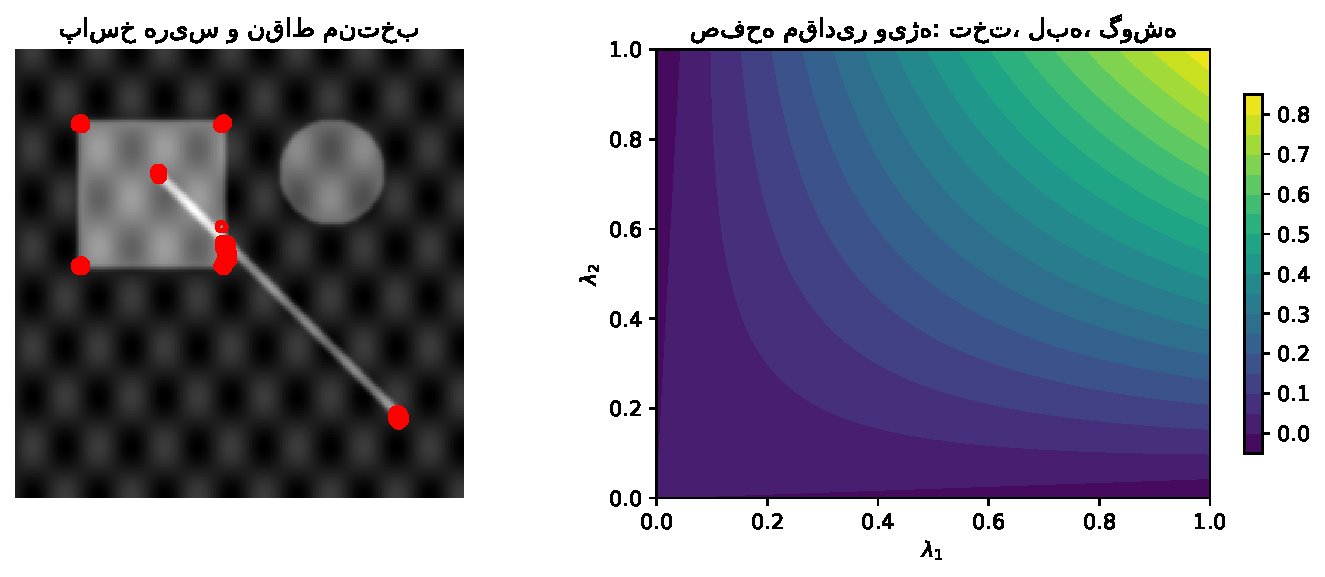
\includegraphics[width=0.95\textwidth]{fig09_02_harris.pdf}
\caption{چپ: نقاط با پاسخ Harris زیاد. راست: پاسخ در صفحه مقادیر ویژه؛ گوشه هنگامی پدید می‌آید که هر دو eigenvalue بزرگ باشند.}
\label{fig:harris}
\end{figure}

\begin{algorithmbox}{الگوریتم 9.1 ـ Harris با non-maximum suppression}
\begin{enumerate}
\item تصویر را در مقیاس مشتق $\sigma_d$ هموار و $I_x,I_y$ را محاسبه کنید.
\item $I_x^2,I_y^2,I_xI_y$ را در مقیاس integration $\sigma_i$ هموار کنید.
\item برای هر پیکسل $R_H=\det M-k(\trace M)^2$ را بسازید.
\item نقاط با $R_H>\tau$ را نگه دارید.
\item در همسایگی شعاع $r$ فقط بیشینه محلی را حفظ کنید.
\item برای دقت زیرپیکسلی، یک تابع درجه دوم روی پاسخ اطراف قله برازش کنید.
\end{enumerate}
پیچیدگی با فیلتر separable و NMS محلی $O(N)$ است. آستانه مطلق بین تصاویر قابل انتقال نیست؛ quantile یا budget ثابت نقاط
برای آزمایش منصفانه مناسب‌تر است.
\end{algorithmbox}

\subsection{FAST و AGAST: تصمیم روی دایره}
FAST به‌جای تانسور، شانزده پیکسل روی دایره Bresenham شعاع ۳ را آزمون می‌کند. نقطه گوشه است اگر حداقل $n$ پیکسل متوالی
از مرکز به اندازه $t$ روشن‌تر یا تاریک‌تر باشند. تصمیم درختی ترتیب آزمون‌ها را برای رد سریع نامزدها می‌آموزد. FAST بسیار
سریع است، اما مقیاس و جهت را ذاتاً فراهم نمی‌کند. ORB با هرم، orientation و NMS آن را به آشکارساز کامل‌تری تبدیل می‌کند
\cite{rosten2006,rublee2011}. AGAST درخت تصمیم را برای معماری‌ها و الگوهای مختلف تعمیم می‌دهد.

\begin{warningbox}
آستانه FAST یا Harris را روی تصویر uint8 و float با یک عدد ثابت استفاده نکنید. مقیاس intensity، gamma و preprocessing
مستقیماً پاسخ را عوض می‌کند. قرارداد داده باید در API آشکارساز صریح باشد.
\end{warningbox}

\section{فضای مقیاس: چرا یک نقطه باید اندازه داشته باشد؟}
یک گوشه در تصویر نزدیک ممکن است در تصویر دور به لکه‌ای کوچک تبدیل شود. آشکارسازی در یک مقیاس ثابت نمی‌تواند زیر zoom تکرارپذیر باشد.
فضای مقیاس خطی با convolution گاوسی تعریف می‌شود:
\begin{equation}
L(\vect x,\sigma)=G(\vect x;\sigma)*I(\vect x),\qquad
G(\vect x;\sigma)=\frac{1}{2\pi\sigma^2}
\exp\!\left(-\frac{\norm{\vect x}^2}{2\sigma^2}\right).
\label{eq:scale_space}
\end{equation}
گاوسی تحت اصول خطی‌بودن، ناوردایی انتقال، نیم‌گروه و عدم ایجاد ساختار جدید، هسته طبیعی فضای مقیاس است.
خاصیت نیم‌گروه
\begin{equation}
G(\cdot;\sigma_1)*G(\cdot;\sigma_2)=
G\!\left(\cdot;\sqrt{\sigma_1^2+\sigma_2^2}\right)
\end{equation}
اجازه می‌دهد octaveها به‌صورت بازگشتی ساخته شوند.

\subsection{نرمال‌سازی مشتق}
مقدار مشتق با بزرگ‌شدن $\sigma$ کاهش می‌یابد. برای مقایسه میان مقیاس‌ها از مشتق نرمال‌شده
\begin{equation}
\partial_{\xi_i}=\sigma^\gamma\partial_{x_i}
\end{equation}
استفاده می‌شود. برای blob دوبعدی، لاپلاسی نرمال‌شده
\begin{equation}
\mathcal L(\vect x,\sigma)=\sigma^2\nabla^2L(\vect x,\sigma)
\label{eq:norm_log}
\end{equation}
در مقیاس متناسب با اندازه blob اکسترمم دارد. این اصل «انتخاب مقیاس خودکار» است.

\subsection{DoG به‌عنوان تقریب LoG}
از معادله گرما داریم
\begin{equation}
\frac{\partial G}{\partial \sigma}=\sigma\nabla^2G.
\end{equation}
پس برای $k$ نزدیک یک:
\begin{align}
G(k\sigma)-G(\sigma)
&\approx (k-1)\sigma\frac{\partial G}{\partial\sigma}\\
&=(k-1)\sigma^2\nabla^2G.
\end{align}
بنابراین Difference of Gaussians
\begin{equation}
D(\vect x,\sigma)=L(\vect x,k\sigma)-L(\vect x,\sigma)
\end{equation}
تقریبی مقیاس‌نرمال از LoG است و با تفریق دو تصویر هموارشده ارزان محاسبه می‌شود. SIFT اکسترمم $D$ را در 26 همسایه فضای
$x,y,\sigma$ می‌یابد \cite{lowe2004}.

\begin{figure}[H]
\centering
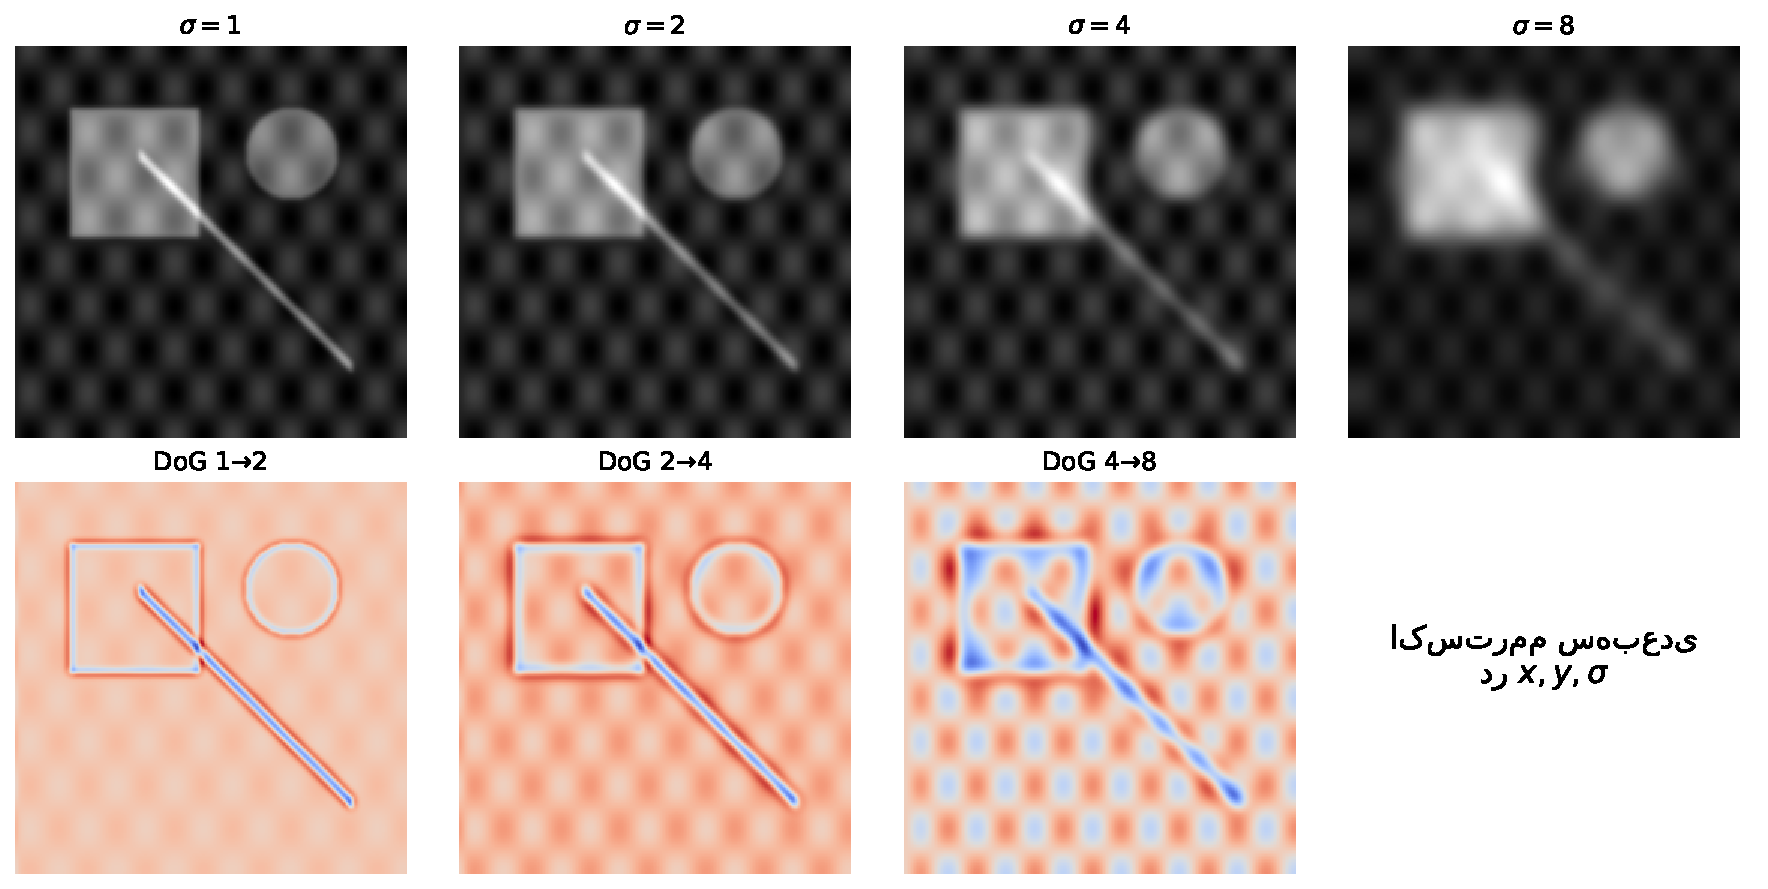
\includegraphics[width=0.97\textwidth]{fig09_03_scale_space.pdf}
\caption{ردیف بالا: تصویر در مقیاس‌های افزاینده. ردیف پایین: DoG میان مقیاس‌های مجاور. نقطه مقیاس‌ناوردا باید در فضای سه‌بعدی مکان--مقیاس اکسترمم باشد.}
\label{fig:scale}
\end{figure}

\subsection{مکان‌یابی زیرپیکسلی و حذف پاسخ لبه}
بردار offset اکسترمم با بسط درجه دوم DoG حول نمونه $\vect z=(x,y,\sigma)$ به دست می‌آید:
\begin{equation}
D(\vect z+\Delta\vect z)\approx D(\vect z)+
\nabla D\trans\Delta\vect z+\frac12\Delta\vect z\trans\mat H_D\Delta\vect z.
\end{equation}
شرط ایستایی می‌دهد
\begin{equation}
\widehat{\Delta\vect z}=-\mat H_D^{-1}\nabla D.
\label{eq:subpixel}
\end{equation}
اگر offset بزرگ باشد، نامزد به نمونه مجاور منتقل و دوباره برازش می‌شود. کنتراست پایین با مقدار interpolated حذف می‌شود.
برای رد پاسخ‌های کشیده روی لبه، اگر $\alpha\ge\beta$ eigenvalueهای Hessian مکانی باشند و $r=\alpha/\beta$، آنگاه
\begin{equation}
\frac{\trace(H)^2}{\det(H)}=\frac{(\alpha+\beta)^2}{\alpha\beta}
=\frac{(r+1)^2}{r}.
\end{equation}
نامزدهایی که این نسبت از حد متناظر $r_{\max}$ بزرگ‌تر است رد می‌شوند.

\subsection{Hessian و blob detector}
Hessian تصویر
\begin{equation}
\mat H_L=
\begin{bmatrix}L_{xx}&L_{xy}\\L_{xy}&L_{yy}\end{bmatrix}
\end{equation}
و پاسخ مقیاس‌نرمال آن
\begin{equation}
R_{\mathrm{Hess}}(\vect x,\sigma)=\sigma^4\det(\mat H_L)
\end{equation}
به ساختارهای blob حساس است. SURF پاسخ Hessian را با box filter و تصویر انتگرالی تقریب می‌کند. KAZE و AKAZE به‌جای فضای
مقیاس گاوسی خطی، diffusion غیرخطی را به‌کار می‌گیرند تا مرزها بهتر حفظ شوند؛ AKAZE با Fast Explicit Diffusion هزینه را
کاهش می‌دهد \cite{alcantarilla2012,alcantarilla2013}.

\subsection{هم‌وردایی آفین و نواحی پایدار}
تغییر دیدگاه محلی تقریباً آفین است. Harris--Affine و Hessian--Affine شکل بیضی ناحیه را با iteration ماتریس second moment
نرمال می‌کنند. MSER مجموعه‌های تراز شدت را دنبال می‌کند و نواحی‌ای را برمی‌گزیند که مساحتشان در بازه threshold کم تغییر کند:
\begin{equation}
q(i)=\frac{|Q_{i+\Delta}\setminus Q_{i-\Delta}|}{|Q_i|}.
\end{equation}
کمینه‌های $q(i)$ نواحی maximally stable هستند. این روش برای نوشته، نماهای شهری و ساختارهای دارای contrast پایدار مفید است
\cite{matas2004}. ارزیابی جامع نواحی affine-covariant نشان داد که انتخاب detector و descriptor باید جداگانه سنجیده شود
\cite{mikolajczyk2005,mikolajczyk2006}.

\begin{algorithmbox}{الگوریتم 9.2 ـ آشکارسازی اکسترمم فضای مقیاس}
\begin{enumerate}
\item برای هر octave، $s+3$ تصویر گاوسی با نسبت $k=2^{1/s}$ بسازید.
\item تصاویر مجاور را تفریق و $s+2$ لایه DoG تولید کنید.
\item هر نمونه داخلی را با ۸ همسایه همان مقیاس و ۹+۹ همسایه مقیاس مجاور مقایسه کنید.
\item نامزد را با معادله \eqref{eq:subpixel} زیرپیکسلی کنید.
\item نامزدهای کنتراست پایین و edge-like را حذف کنید.
\item مختصات را به دستگاه تصویر اصلی و مقیاس فیزیکی تبدیل کنید.
\end{enumerate}
اگر kernelها separable باشند، ساخت pyramid نسبت به تعداد پیکسل‌های کل octaveها خطی است. هزینه اصلی descriptor و matching است، نه صرفاً DoG.
\end{algorithmbox}

\section{تخصیص جهت و نرمال‌سازی ناحیه}
برای ناوردایی دوران، gradientهای اطراف keypoint در مقیاس انتخاب‌شده محاسبه می‌شوند:
\begin{equation}
m(\vect x)=\sqrt{L_x^2+L_y^2},\qquad
\theta(\vect x)=\operatorname{atan}(L_y,L_x).
\end{equation}
هر نمونه با وزن گاوسی به histogram جهت رأی می‌دهد. قله اصلی جهت canonical را تعیین می‌کند؛ قله‌های نزدیک به قله اصلی می‌توانند
keypoint اضافی بسازند. سپس patch به دستگاه محلی
\begin{equation}
\vect x'=\frac{1}{\sigma}\mat R(-\theta)(\vect x-\vect x_0)
\end{equation}
منتقل می‌شود. این مرحله آشکارساز هم‌وردا را به support region نرمال تبدیل می‌کند.

\begin{warningbox}
جهت‌گذاری در ساختارهای متقارن ناپایدار است. یک دایره یا بافت isotropic جهت یکتا ندارد. تولید چند orientation پوشش را افزایش می‌دهد،
اما تعداد descriptor و تطابق کاذب را نیز زیاد می‌کند. ambiguity باید در طراحی matcher لحاظ شود.
\end{warningbox}

\section{توصیفگرهای محلی: چه چیزی از وصله باقی بماند؟}
توصیفگر تابعی از patch نرمال‌شده است:
\begin{equation}
\vect d=\Psi\!\left(\mathcal W(I;\vect p,\sigma,\theta,\mat A)\right)\in\R^D
\quad\text{یا}\quad \{0,1\}^D.
\end{equation}
سه trade-off بنیادی‌اند: localization در برابر pooling، ناوردایی در برابر تمایزبخشی، و ابعاد در برابر سرعت جست‌وجو.

\subsection{وصله خام، whitening و NCC}
ساده‌ترین descriptor بردار پیکسل‌های وصله است. پس از حذف میانگین و نرمال‌سازی $\ell_2$، فاصله اقلیدسی و correlation به هم مرتبط‌اند:
\begin{equation}
\norm{\widehat{\vect p}-\widehat{\vect q}}_2^2
=2-2\widehat{\vect p}\trans\widehat{\vect q}.
\end{equation}
whitening با کوواریانس داده
\begin{equation}
\vect z=\mat\Sigma^{-1/2}(\vect p-\vect\mu)
\end{equation}
جهت‌های پرتکرار و پرهمبستگی را متعادل می‌کند، اما نسبت به misalignment حساس است.

\subsection{SIFT: histogram جهت با pooling مکانی}
SIFT یک پنجره معمولاً $16\times16$ را به $4\times4$ سلول تقسیم و در هر سلول histogram هشت‌جهتی می‌سازد؛ در نتیجه
$4\times4\times8=128$ بعد دارد. رأی هر gradient به‌صورت trilinear میان دو سلول مکانی و دو bin جهت پخش می‌شود تا تغییر کوچک مکان
یا جهت descriptor را ناگهانی عوض نکند. بردار سپس:
\begin{enumerate}
\item با نرم $\ell_2$ نرمال می‌شود؛
\item مؤلفه‌ها در حدی مانند $0.2$ clip می‌شوند؛
\item دوباره نرمال می‌شود.
\end{enumerate}
clip اثر gradientهای بسیار غالب و تغییر illumination موضعی را کاهش می‌دهد.

\begin{figure}[H]
\centering
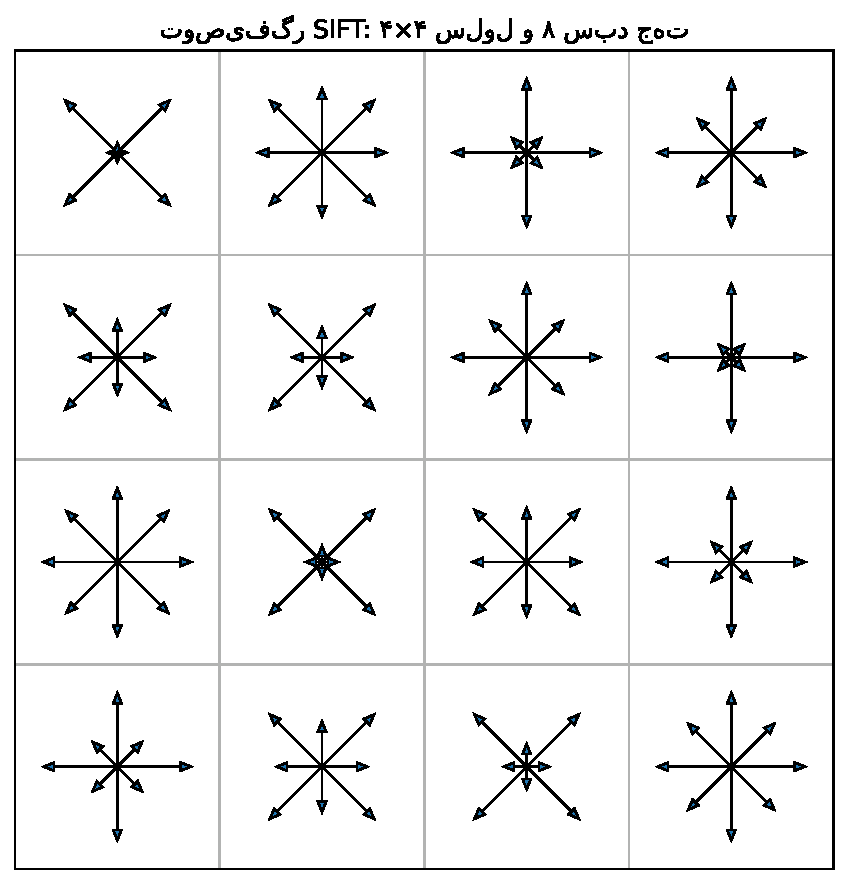
\includegraphics[width=0.62\textwidth]{fig09_04_sift_descriptor.pdf}
\caption{نمای آموزشی descriptor SIFT. pooling جهت در سلول‌های مکانی، کمی خطای localization را تحمل می‌کند و در عین حال آرایش محلی را نگه می‌دارد.}
\label{fig:sift_desc}
\end{figure}

\begin{proofbox}[چرا histogram نسبت به جابه‌جایی کوچک پایدارتر از پیکسل خام است؟]
اگر gradient از مختصات $\vect x$ به $\vect x+\Delta\vect x$ جابه‌جا شود، رأی trilinear به‌طور پیوسته میان سلول‌ها بازتوزیع می‌شود.
در patch خام، همان جابه‌جایی می‌تواند مؤلفه‌ای را از یک index به index دیگر منتقل کند و فاصله بزرگی بسازد. pooling یک low-pass در فضای
مکان--جهت است؛ پایداری می‌خرد، اما جزئیات فرکانس بالا را حذف می‌کند.
\end{proofbox}

\subsection{RootSIFT و هندسه Hellinger}
اگر histogram غیرمنفی $\vect h$ باشد، RootSIFT ابتدا $\ell_1$ نرمال و سپس ریشه مؤلفه‌ای می‌گیرد:
\begin{equation}
\vect r_i=\sqrt{\frac{h_i}{\sum_j h_j+\varepsilon}}.
\end{equation}
فاصله اقلیدسی میان $\vect r$ها معادل فاصله Hellinger میان histogramهاست. این تغییر ساده اغلب matching و retrieval را بهبود می‌دهد
\cite{arandjelovic2012}.

\subsection{HOG: توصیف dense برای بازشناسی}
HOG همان ایده histogram جهت را به شبکه dense سلول‌ها و block normalization گسترش می‌دهد. برای block بردار $\vect v$، نرمال‌سازی L2-Hys:
\begin{equation}
\vect v\leftarrow\frac{\vect v}{\sqrt{\norm{\vect v}_2^2+\varepsilon^2}},
\quad v_i\leftarrow\min(v_i,c),
\quad \vect v\leftarrow\frac{\vect v}{\sqrt{\norm{\vect v}_2^2+\varepsilon^2}}.
\end{equation}
HOG+linear SVM نمونه کلاسیک تبدیل gradient محلی به detector شیء است \cite{dalal2005}.

\subsection{Shape Context و descriptor شکل}
برای نقطه مرزی $p_i$، توزیع نسبی سایر نقاط در binهای log-polar ثبت می‌شود:
\begin{equation}
h_i(k)=\#\{q\ne p_i:q-p_i\in\text{bin}(k)\}.
\end{equation}
هزینه تطبیق دو histogram با $\chi^2$:
\begin{equation}
C_{ij}=\frac12\sum_k\frac{(h_i(k)-h_j(k))^2}{h_i(k)+h_j(k)+\varepsilon}.
\end{equation}
سپس assignment و spline تغییر شکل را برآورد می‌کند. این روش برای contour و بازشناسی شکل کلاسیک مهم است \cite{belongie2002}.

\subsection{توصیفگرهای دودویی}
BRIEF مجموعه آزمون‌های شدت است:
\begin{equation}
\tau(\vect p;\vect a_i,\vect b_i)=
\begin{cases}
1,&I(\vect p+\vect a_i)<I(\vect p+\vect b_i),\\
0,&\text{otherwise}.
\end{cases}
\end{equation}
رشته $D$ بیتی با XOR و popcount بسیار سریع مقایسه می‌شود:
\begin{equation}
\Hamm(\vect b,\vect c)=\sum_{i=1}^D b_i\oplus c_i.
\end{equation}
BRIEF ذاتاً rotation invariant نیست. ORB جهت را با intensity centroid برآورد و الگوی آزمون را می‌چرخاند؛ همچنین زوج آزمون‌های پُرواریانس و
کم‌همبستگی را انتخاب می‌کند \cite{calonder2010,rublee2011}. BRISK از sampling pattern حلقوی و FREAK از الگوی شبیه شبکیه استفاده می‌کنند.
AKAZE descriptor دودویی M-LDB را روی فضای مقیاس غیرخطی می‌سازد.

\begin{figure}[H]
\centering
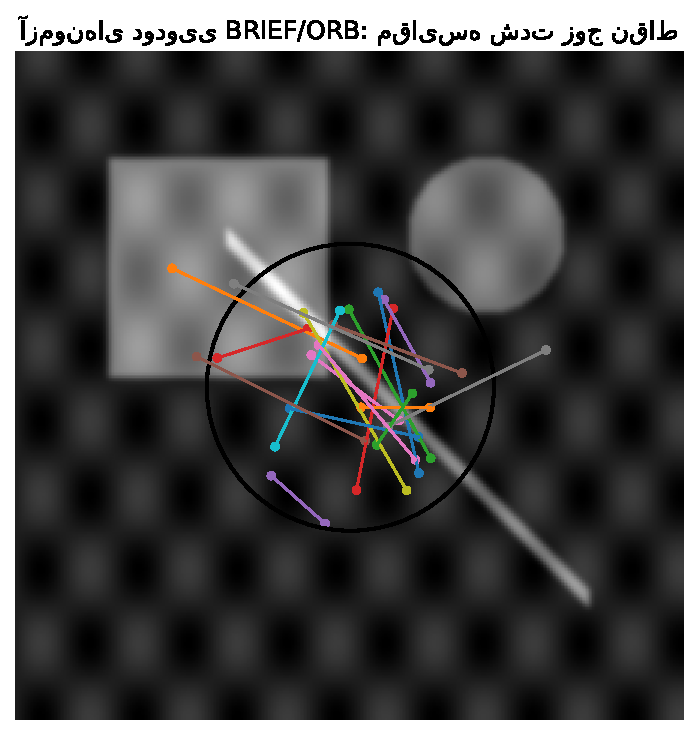
\includegraphics[width=0.72\textwidth]{fig09_05_binary_tests.pdf}
\caption{نمای شماتیک آزمون‌های زوجی شدت در توصیفگر دودویی. سرعت بالا نتیجه تبدیل descriptor به رشته بیت و فاصله به popcount است.}
\label{fig:binary}
\end{figure}

\begin{longtable}{p{25mm}p{27mm}p{27mm}p{31mm}p{29mm}}
\toprule
توصیفگر & نوع & فاصله معمول & نقطه قوت & محدودیت اصلی \\
\midrule
SIFT/RootSIFT & حقیقی، ۱۲۸بعد & $\ell_2$/Hellinger & robust و متمایز & هزینه و حافظه بیشتر \\
HOG & حقیقی، dense & خطی/SVM & شکل و gradient & ناوردایی محدود دیدگاه \\
BRIEF & دودویی & Hamming & بسیار سریع & بدون جهت/مقیاس ذاتی \\
ORB & دودویی & Hamming & real-time، آزاد و در دسترس & در تغییر دید شدید ضعیف‌تر از SIFT \\
BRISK/FREAK & دودویی & Hamming & الگوی نمونه‌برداری کارا & حساس به blur و photometric shift \\
AKAZE & دودویی/حقیقی & Hamming/$\ell_2$ & scale-space لبه‌نگهدار & تنظیمات و هزینه diffusion \\
Shape Context & histogram & $\chi^2$ & شکل و deformable matching & نیاز به contour/assignment \\
\bottomrule
\end{longtable}

\section{تطبیق توصیفگر: از فاصله تا correspondence}
برای descriptorهای query $\{\vect d_i\}$ و database $\{\vect e_j\}$، تطبیق خام
\begin{equation}
\pi(i)=\argmin_j d(\vect d_i,\vect e_j)
\end{equation}
است. اما «نزدیک‌ترین» الزاماً «درست» نیست؛ در هر پایگاه داده یک نزدیک‌ترین همسایه وجود دارد، حتی اگر هیچ correspondence واقعی نباشد.

\subsection{انتخاب معیار فاصله}
\begin{align}
d_2(\vect x,\vect y)&=\norm{\vect x-\vect y}_2,\\
d_{\cos}(\vect x,\vect y)&=1-\frac{\vect x\trans\vect y}{\norm{\vect x}\norm{\vect y}},\\
d_M(\vect x,\vect y)&=\sqrt{(\vect x-\vect y)\trans\mat M(\vect x-\vect y)},\\
d_H(\vect b,\vect c)&=\sum_i b_i\oplus c_i.
\end{align}
برای descriptorهای $\ell_2$-نرمال، فاصله اقلیدسی و cosine ranking یکسان می‌دهند. Mahalanobis correlation و اهمیت ابعاد را مدل می‌کند، اما
نیازمند برآورد یا یادگیری $\mat M\succeq0$ است. استفاده Hamming برای descriptor float یا $\ell_2$ برای بیت‌ها خطای مفهومی است.

\subsection{آزمون نسبت Lowe}
اگر $d_1$ و $d_2$ فاصله نخستین و دومین همسایه باشند، تطابق پذیرفته می‌شود اگر
\begin{equation}
\frac{d_1}{d_2}<\rho.
\label{eq:ratio}
\end{equation}
شهود: تطابق درست باید نه‌فقط نزدیک، بلکه نسبت به گزینه جایگزین متمایز باشد. threshold ثابت مثل $0.7$ یا $0.8$ قانون جهان‌شمول نیست؛ به descriptor،
دامنه، تعداد ویژگی و recall مورد نیاز وابسته است. مقاله SIFT این آزمون را برای کاهش background clutter به‌کار برد \cite{lowe2004}.

\begin{figure}[H]
\centering
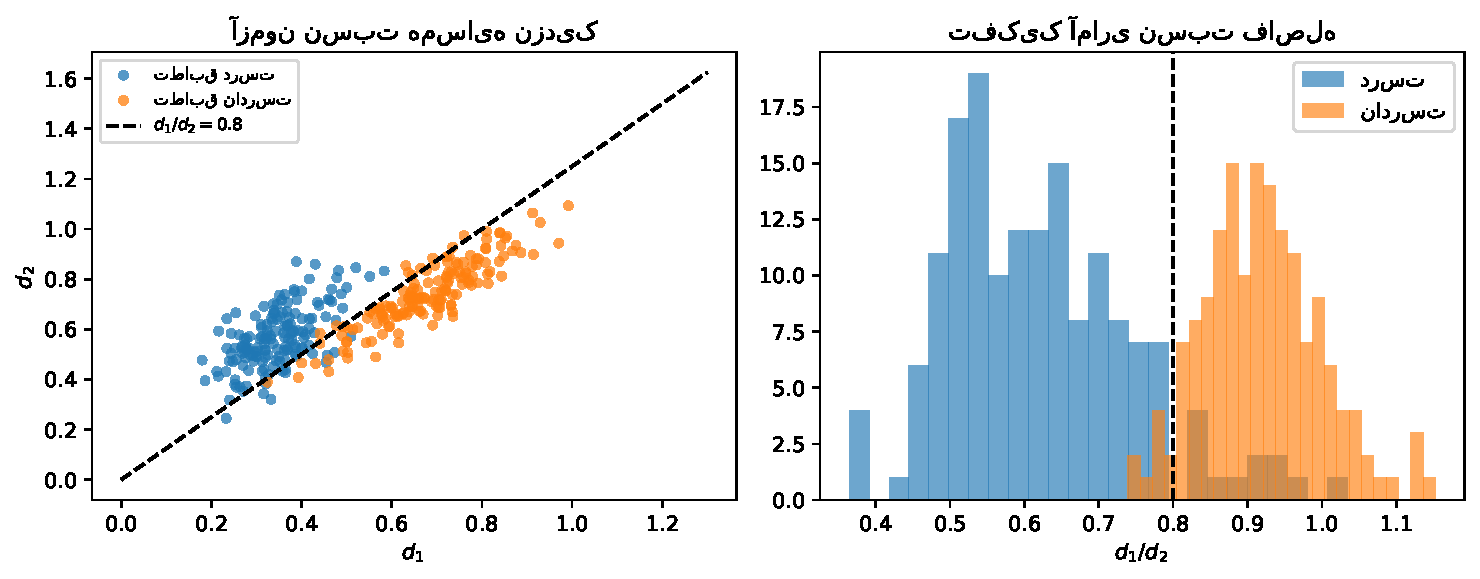
\includegraphics[width=0.96\textwidth]{fig09_06_ratio_test.pdf}
\caption{آزمون نسبت. تطابق درست معمولاً فاصله اول کوچک و فاصله دوم به‌وضوح بزرگ‌تری دارد؛ بافت تکراری دو همسایه تقریباً برابر می‌سازد.}
\label{fig:ratio}
\end{figure}

\subsection{cross-check، mutual nearest neighbor و uniqueness}
تطابق mutual اگر
\begin{equation}
\pi_{A\to B}(i)=j,\qquad \pi_{B\to A}(j)=i
\end{equation}
باشد. این آزمون precision را افزایش و recall را کاهش می‌دهد. در stereo rectified می‌توان علاوه بر mutuality، محدودیت disparity و ordering را وارد کرد.
در retrieval، یک descriptor database ممکن است به چند query پاسخ دهد؛ assignment یک‌به‌یک را می‌توان با الگوریتم Hungarian روی ماتریس هزینه حل کرد، اما
$O(n^3)$ و حساس به unmatched points است. formulation با dummy node یا optimal transport unbalanced انعطاف بیشتری دارد.

\subsection{جست‌وجوی دقیق و تقریبی}
brute-force برای $N_qN_dD$ عملیات ساده و برای مجموعه کوچک قابل اعتماد است. برای مقیاس بزرگ:
\begin{itemize}
\item kd-tree در ابعاد پایین مفید، اما در ابعاد زیاد دچار curse of dimensionality می‌شود؛
\item randomized kd-trees و hierarchical k-means در FLANN trade-off جست‌وجو/دقت می‌دهند؛
\item LSH برای رشته‌های دودویی یا فضاهای metric خاص مناسب است؛
\item product quantization بردار را به زیر‌بردار تقسیم و فاصله تقریبی را با lookup table محاسبه می‌کند؛
\item inverted file ابتدا coarse cell را انتخاب و سپس PQ را در همان cell اجرا می‌کند.
\end{itemize}
مستندات OpenCV نیز L2 را برای SIFT/SURF و Hamming را برای descriptorهای دودویی تفکیک می‌کند \cite{opencvfeatures2026}.

\begin{algorithmbox}{الگوریتم 9.3 ـ تطبیق مقاوم اولیه}
\begin{enumerate}
\item نوع descriptor و metric سازگار را تعیین کنید.
\item برای هر query دو همسایه نزدیک را پیدا کنید.
\item ratio test با $\rho$ ازپیش‌اعلام‌شده اعمال کنید.
\item در صورت نیاز mutual cross-check را اجرا کنید.
\item duplicateهای مکانی یا چند orientation یک keypoint را ادغام کنید.
\item score، index، مختصات، scale و orientation هر match را نگه دارید؛ فقط تصویر ترسیمی کافی نیست.
\item تطابق‌ها را به مرحله هندسی تحویل دهید؛ پیش از هندسه نتیجه object detection اعلام نکنید.
\end{enumerate}
\end{algorithmbox}

\begin{workshopbox}[SIFT/ORB و انتخاب matcher]
\begin{latin}
\begin{lstlisting}
import cv2 as cv

def detect_and_match(img1, img2, method="sift", ratio=0.75):
    if method == "sift":
        detector = cv.SIFT_create(nfeatures=3000)
        norm = cv.NORM_L2
    elif method == "orb":
        detector = cv.ORB_create(nfeatures=3000, scaleFactor=1.2, nlevels=8)
        norm = cv.NORM_HAMMING
    else:
        raise ValueError("method must be 'sift' or 'orb'")

    k1, d1 = detector.detectAndCompute(img1, None)
    k2, d2 = detector.detectAndCompute(img2, None)
    if d1 is None or d2 is None:
        return k1, k2, []

    matcher = cv.BFMatcher(normType=norm, crossCheck=False)
    pairs = matcher.knnMatch(d1, d2, k=2)
    good = [m for m, n in pairs if m.distance < ratio * n.distance]
    return k1, k2, good
\end{lstlisting}
\end{latin}
برای گزارش علمی، علاوه بر تعداد good match، تعداد inlier پس از مدل هندسی، reprojection error، زمان detect/describe/match و حافظه descriptor را ذخیره کنید.
\end{workshopbox}

\section{راستی‌آزمایی هندسی: شباهت توصیفگر کافی نیست}
تطابق‌های اولیه مجموعه‌ای از زوج نقاط $\{(\vect x_i,\vect x'_i)\}$ است. مدل هندسی $\mat\theta$ residual
\begin{equation}
r_i(\mat\theta)=d_g\!\left(\vect x'_i,f(\vect x_i;\mat\theta)\right)
\end{equation}
می‌سازد. برای homography از خطای symmetric transfer، برای fundamental matrix از Sampson و برای PnP از reprojection استفاده می‌شود.

\begin{figure}[H]
\centering
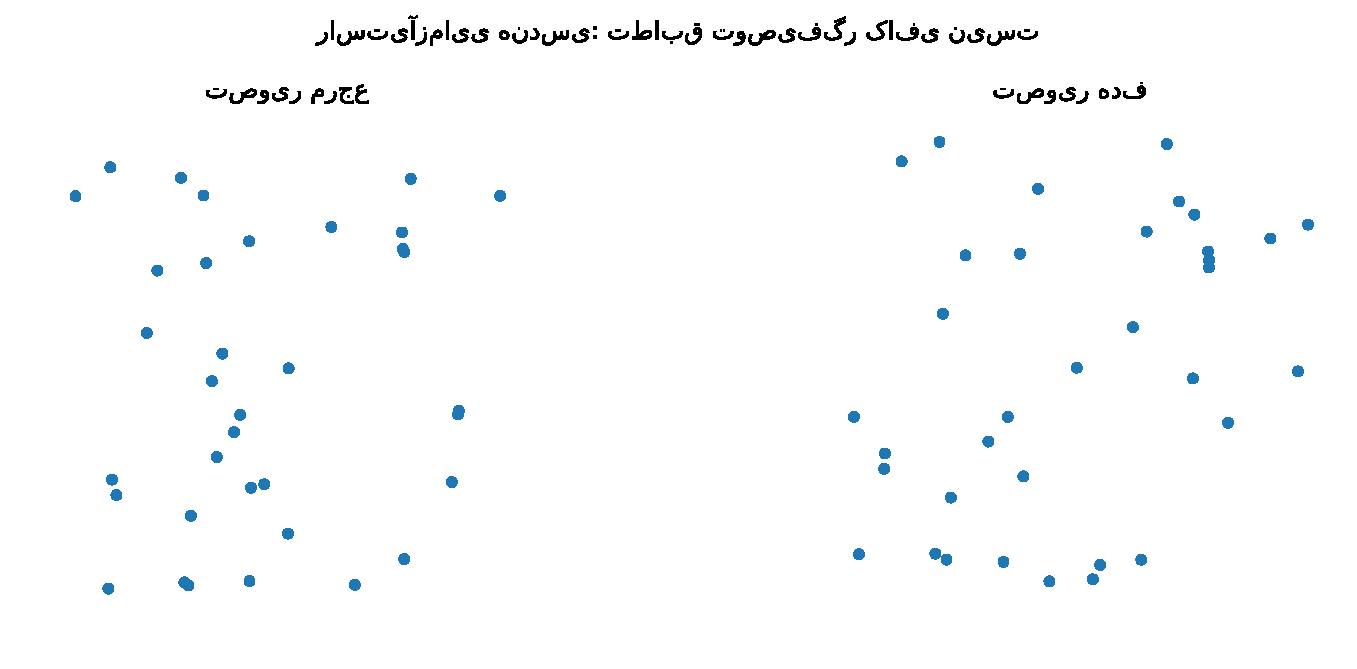
\includegraphics[width=0.88\textwidth]{fig09_08_geometric_verification.pdf}
\caption{وجود matchهای descriptor تنها فرضیه می‌سازد. مدل هندسی باید سازگاری جمعی correspondenceها را بررسی کند.}
\label{fig:geom}
\end{figure}

\subsection{RANSAC و احتمال موفقیت}
اگر سهم inlier برابر $w$ و اندازه minimal sample برابر $s$ باشد، احتمال اینکه یک sample کاملاً inlier باشد $w^s$ است. پس احتمال شکست پس از $N$ iteration:
\begin{equation}
P_{\mathrm{fail}}=(1-w^s)^N.
\end{equation}
برای احتمال موفقیت $p$:
\begin{equation}
N\ge \frac{\log(1-p)}{\log(1-w^s)}.
\label{eq:ransac_iters}
\end{equation}
مثلاً با $w=0.5$، homography با $s=4$ و $p=0.99$ حدود ۷۲ iteration می‌خواهد؛ با $w=0.2$ این عدد به حدود ۲۸۷۶ می‌رسد.
بنابراین کیفیت matching اولیه مستقیماً هزینه هندسه را تعیین می‌کند \cite{fischler1981}.

\begin{figure}[H]
\centering
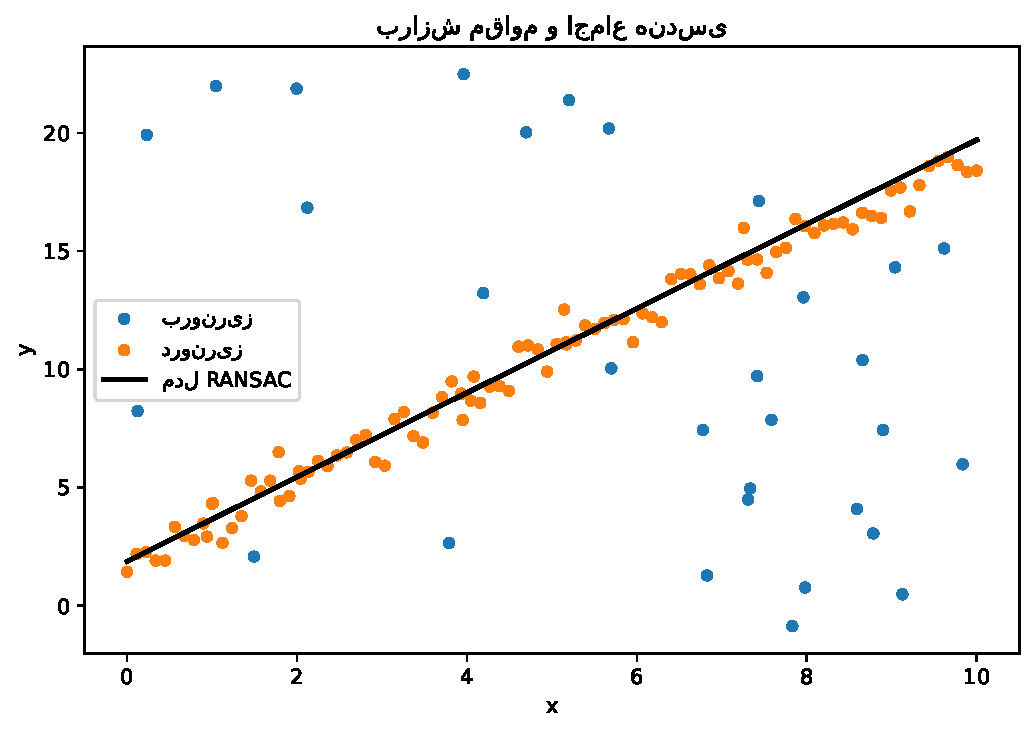
\includegraphics[width=0.72\textwidth]{fig09_07_ransac.pdf}
\caption{RANSAC مدل را از subset حداقلی پیشنهاد و با consensus ارزیابی می‌کند. threshold residual تعریف عملی inlier است.}
\label{fig:ransac}
\end{figure}

\begin{algorithmbox}{الگوریتم 9.4 ـ RANSAC تطبیقی}
\begin{enumerate}
\item $N=N_{\max}$، بهترین score و mask خالی را مقداردهی کنید.
\item یک minimal sample غیرتباه انتخاب و مدل را برازش کنید.
\item residual همه داده‌ها را حساب و inlierهای $r_i<\tau$ را مشخص کنید.
\item مدل را با score robust، نه فقط شمارش خام، رتبه‌بندی کنید.
\item اگر بهتر بود، مدل را روی inlierها پالایش و $\widehat w$ را به‌روزرسانی کنید.
\item $N$ را با معادله \eqref{eq:ransac_iters} و $\widehat w$ کاهش دهید.
\item پس از توقف، nonlinear refinement روی inlierها اجرا و covariance تقریبی گزارش کنید.
\end{enumerate}
\end{algorithmbox}

\subsection{threshold و مدل نویز}
آستانه پیکسلی ثابت با تغییر resolution و uncertainty keypoint عادلانه نیست. اگر covariance residual برابر $\mat\Sigma_i$ باشد، فاصله Mahalanobis
\begin{equation}
r_i^2=\vect e_i\trans\mat\Sigma_i^{-1}\vect e_i
\end{equation}
را با quantile توزیع $\chi^2$ مقایسه می‌کنیم. scale keypoint، localization detector و camera calibration باید در uncertainty وارد شوند.

\subsection{پیشرفت‌های RANSAC}
\begin{itemize}
\item \textbf{PROSAC:} sample را از matchهای با score بهتر آغاز و دامنه را تدریجی گسترش می‌دهد؛
\item \textbf{LO-RANSAC:} هر مدل خوب را با local optimization روی inlierها بهبود می‌دهد؛
\item \textbf{USAC:} sampler، verification، degeneracy و polishing را در چارچوب واحد ترکیب می‌کند؛
\item \textbf{MAGSAC++:} به‌جای threshold نویز ثابت، کیفیت و وزن‌ها را با marginalization روی noise scale و IRLS می‌سازد \cite{barath2020}.
\end{itemize}

\subsection{تباهی و انتخاب مدل}
چهار نقطه تقریباً هم‌خط برای homography تباه‌اند؛ نقاط روی صفحه خاص ممکن است fundamental matrix را با homography اشتباه‌پذیر کنند؛ حرکت دوربین و scene geometry
نیز critical configuration می‌سازد. pipeline حرفه‌ای باید:
\begin{enumerate}
\item minimal sample را پیش از solve از نظر rank/area آزمون کند؛
\item چند مدل محتمل مانند $H$ و $F$ را مقایسه کند؛
\item complexity penalty یا geometric prior داشته باشد؛
\item cheirality و محدودیت‌های دوربین را پس از بازیابی pose بررسی کند.
\end{enumerate}

\begin{keybox}[معیار تصمیم برای کاربرد]
برای panorama صفحه‌ای یا دوران خالص، homography مناسب است؛ برای دو دید عمومی صحنه سه‌بعدی، fundamental/essential؛ برای localization با نقاط سه‌بعدی، PnP؛
و برای جسم non-rigid یک مدل سراسری واحد کافی نیست. انتخاب مدل پیش از RANSAC بخشی از فرض مسئله است.
\end{keybox}

\section{از match به بازشناسی: سه خانواده کلاسیک}
بازشناسی را می‌توان به سه صورت دید:
\begin{enumerate}
\item \textbf{instance recognition:} آیا همین شیء/نما قبلاً دیده شده است؟
\item \textbf{category recognition:} آیا تصویر به کلاس مفهومی تعلق دارد؟
\item \textbf{retrieval:} تصاویر مشابه را با ranking برگردان.
\end{enumerate}
ویژگی محلی برای instance و geometry بسیار طبیعی است؛ category recognition به تجمیع و classifier نیاز دارد.

\subsection{تطبیق مستقیم قالب، chamfer و generalized Hough}
برای edge mapهای template $T$ و تصویر، chamfer distance با distance transform $D_I$:
\begin{equation}
E_{\mathrm{chamfer}}(T,I)=\frac1{|T|}\sum_{\vect x\in T}D_I(\vect x)
\end{equation}
است. نسخه جهت‌دار اختلاف tangent را نیز جریمه می‌کند. Generalized Hough برای هر نقطه مرزی، بردار به مرکز مرجع را در R-table ذخیره و در تصویر جدید در فضای
وضعیت رأی‌گیری می‌کند. این روش برای silhouette مشخص و تعداد کلاس کم تفسیرپذیر است، اما فضای رأی با scale/rotation بزرگ می‌شود.

\subsection{ویژگی‌های کلی شکل و ممان}
ممان‌های هندسی
\begin{equation}
m_{pq}=\sum_x\sum_y x^py^qI(x,y)
\end{equation}
و ممان مرکزی
\begin{equation}
\mu_{pq}=\sum_x\sum_y(x-\bar x)^p(y-\bar y)^qI(x,y)
\end{equation}
برای مرکز، جهت و invariants استفاده می‌شوند. Hu هفت ترکیب ناوردا نسبت به انتقال، scale و rotation ساخت. این توصیفگرها compact و مناسب شکل تمیزند، ولی به segmentation error
و clutter حساس‌اند.

\subsection{PCA و Eigenfaces}
بردار تصویر $\vect x\in\R^D$ حول میانگین مرکز می‌شود. PCA جهت‌های بیشینه واریانس را از eigenvectors کوواریانس
\begin{equation}
\mat S_T=\frac1N\sum_{i=1}^N(\vect x_i-\vect\mu)(\vect x_i-\vect\mu)\trans
\end{equation}
می‌یابد:
\begin{equation}
\mat W_{\mathrm{PCA}}=\argmax_{\mat W\trans\mat W=I}
\trace(\mat W\trans\mat S_T\mat W).
\end{equation}
Eigenfaces تصویر را در subspace کم‌بعد بازنمایی و nearest neighbor را ممکن می‌کند \cite{turk1991}. PCA label را نمی‌بیند؛ تغییر نور ممکن است از تفاوت هویت واریانس بیشتری داشته باشد.

\subsection{LDA و Fisherfaces}
با میانگین کلاس $\mu_c$:
\begin{align}
\mat S_W&=\sum_c\sum_{i:y_i=c}(\vect x_i-\vect\mu_c)(\vect x_i-\vect\mu_c)\trans,\\
\mat S_B&=\sum_cN_c(\vect\mu_c-\vect\mu)(\vect\mu_c-\vect\mu)\trans.
\end{align}
LDA نسبت جدایی بین‌کلاس به درون‌کلاس را بیشینه می‌کند:
\begin{equation}
\mat W_{\mathrm{LDA}}=\argmax_{\mat W}
\frac{|\mat W\trans\mat S_B\mat W|}{|\mat W\trans\mat S_W\mat W|}.
\end{equation}
راه‌حل از مسئله generalized eigenvalue $S_B\vect w=\lambda S_W\vect w$ می‌آید. در $D\gg N$، $S_W$ تکین است و ابتدا PCA یا regularization لازم است
\cite{belhumeur1997}.

\begin{figure}[H]
\centering
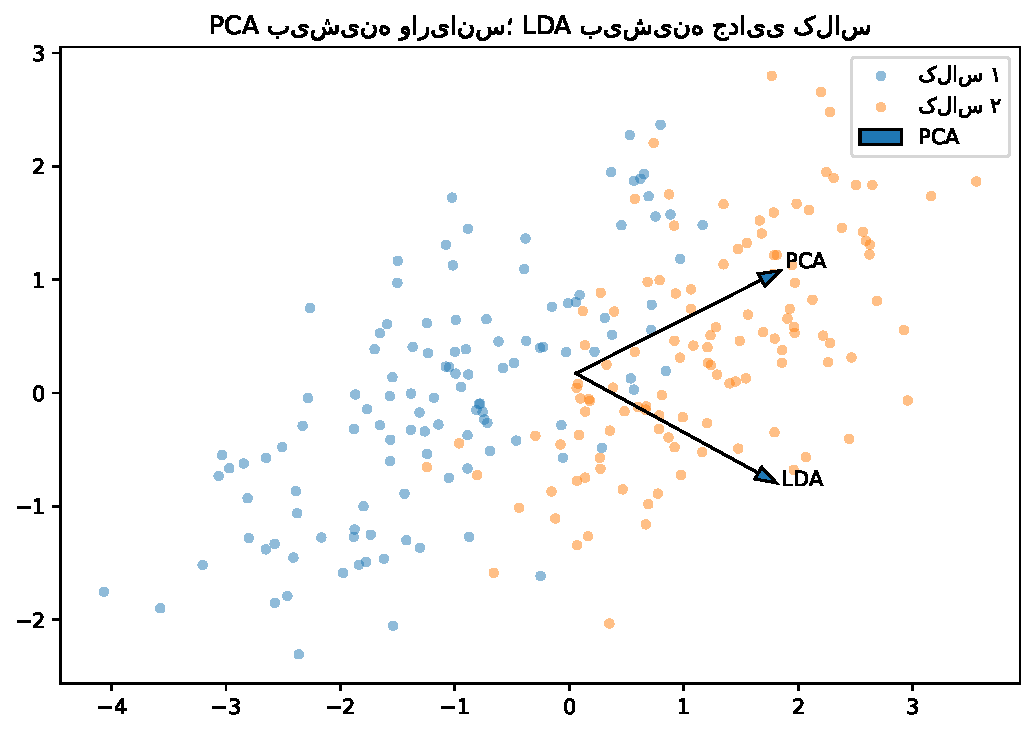
\includegraphics[width=0.73\textwidth]{fig09_11_pca_lda.pdf}
\caption{PCA جهت واریانس کل را می‌گیرد؛ LDA جهت جدایی برچسب‌دار را. هر دو خطی و وابسته به preprocessing و split صحیح‌اند.}
\label{fig:pcalda}
\end{figure}

\section{طبقه‌بندهای کلاسیک روی ویژگی}
\subsection{kNN و هندسه فضای ویژگی}
قاعده نزدیک‌ترین همسایه برای نمونه $\vect x$:
\begin{equation}
\widehat y=\operatorname{mode}\{y_i:i\in\mathcal N_k(\vect x)\}
\end{equation}
است. ساده و بدون آموزش پارامتری است، اما هزینه inference با اندازه داده رشد می‌کند و به scaling ابعاد و curse of dimensionality حساس است.
نسخه وزن‌دار از $w_i=(d_i+\varepsilon)^{-p}$ استفاده می‌کند. انتخاب $k$ باید داخل validation و پس از تمام مراحل feature normalization انجام شود.

\subsection{مدل مولد گاوسی: LDA و QDA به‌عنوان classifier}
اگر
\begin{equation}
p(\vect x\mid y=c)=\mathcal N(\vect x;\vect\mu_c,\mat\Sigma_c),
\end{equation}
آنگاه log-posterior تا ثابت برابر
\begin{equation}
\delta_c(\vect x)=-\frac12\log|\mat\Sigma_c|-\frac12(\vect x-\vect\mu_c)\trans\mat\Sigma_c^{-1}(\vect x-\vect\mu_c)+\log\pi_c.
\end{equation}
است. covariance مشترک مرز خطی LDA و covariance مستقل مرز درجه دوم QDA می‌دهد. shrinkage
\begin{equation}
\widehat\Sigma_\alpha=(1-\alpha)\widehat\Sigma+\alpha\frac{\trace(\widehat\Sigma)}{D}\mat I
\end{equation}
برای داده کم و feature پر‌بعد ضروری است.

\subsection{ماشین بردار پشتیبان}
برای داده دودویی $(\vect x_i,y_i)$، soft-margin SVM:
\begin{equation}
\min_{\vect w,b,\vect\xi}\frac12\norm{\vect w}_2^2+C\sum_i\xi_i
\quad\text{s.t.}\quad
y_i(\vect w\trans\vect x_i+b)\ge1-\xi_i,
\quad \xi_i\ge0.
\label{eq:svm_primal}
\end{equation}
فاصله مرز تا نزدیک‌ترین نمونه‌ها $2/\norm{\vect w}$ است؛ کمینه‌کردن نرم، حاشیه را بیشینه می‌کند. دوگان:
\begin{equation}
\max_{\vect\alpha}\sum_i\alpha_i-\frac12\sum_{i,j}\alpha_i\alpha_jy_iy_jK(\vect x_i,\vect x_j),
\quad 0\le\alpha_i\le C,
\quad \sum_i\alpha_iy_i=0.
\end{equation}
تنها نمونه‌های $\alpha_i>0$ بردار پشتیبان‌اند. برای histogramها، kernelهای $\chi^2$ یا intersection می‌توانند مناسب‌تر از RBF باشند، اما linear SVM روی HOG، VLAD و FV پس از
نرمال‌سازی اغلب baseline قوی و سریع است \cite{cortes1995,dalal2005}.

\begin{figure}[H]
\centering
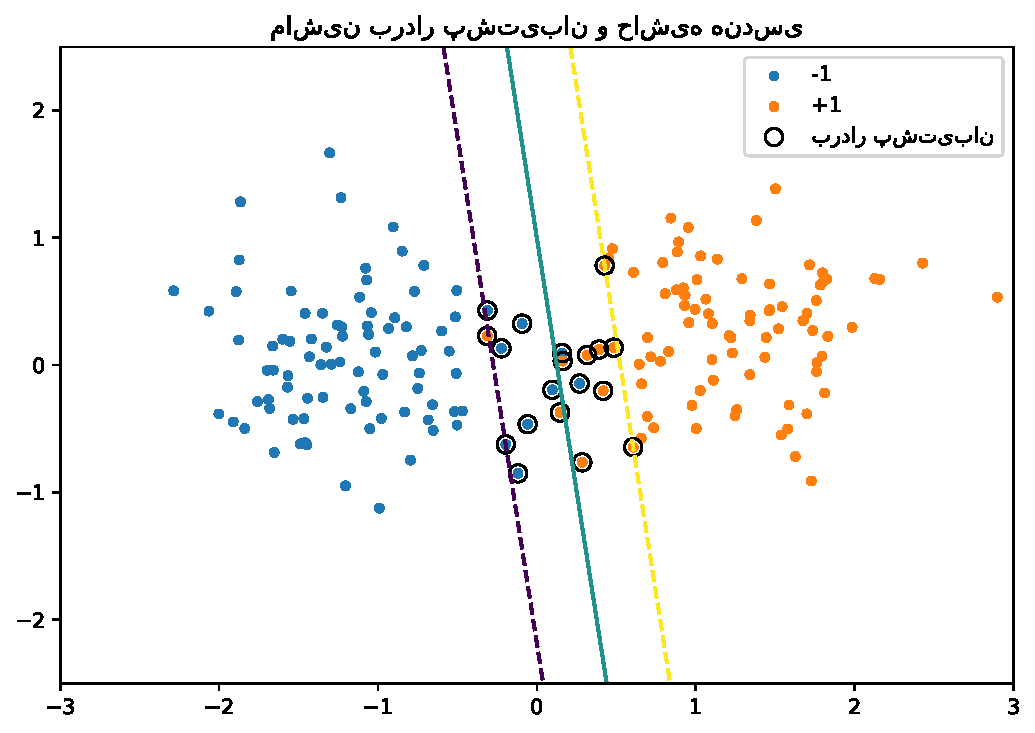
\includegraphics[width=0.72\textwidth]{fig09_12_svm.pdf}
\caption{SVM خطی. بردارهای پشتیبان مرز را تعیین می‌کنند؛ نقاط دورتر در جواب primal اثر مستقیم ندارند.}
\label{fig:svm}
\end{figure}

\subsection{چندکلاسه و calibration}
راهبردهای one-vs-rest و one-vs-one چند classifier دودویی می‌سازند. score حاشیه احتمال نیست. Platt scaling مدل logistic
\begin{equation}
P(y=1\mid f)=\frac{1}{1+\exp(Af+B)}
\end{equation}
را روی validation جدا برازش می‌کند؛ isotonic regression انعطاف‌پذیرتر اما پرریسک‌تر است. calibration set نباید با test یکی باشد.

\subsection{AdaBoost و cascade}
برای weak learnerهای $h_t(\vect x)\in\{-1,+1\}$، AdaBoost classifier
\begin{equation}
F_T(\vect x)=\sum_{t=1}^T\alpha_th_t(\vect x)
\end{equation}
و زیان نمایی
\begin{equation}
\sum_i\exp\left(-y_iF_T(\vect x_i)\right)
\end{equation}
را به‌صورت stagewise کاهش می‌دهد. وزن نمونه‌ها
\begin{equation}
w_i^{(t+1)}\propto w_i^{(t)}\exp(-\alpha_ty_ih_t(\vect x_i))
\end{equation}
نمونه‌های اشتباه را تقویت می‌کند. Viola--Jones از Haar-like featureهای سریع با integral image و cascade استفاده کرد: stageهای نخست تقریباً همه پنجره‌های منفی آسان را با هزینه کم رد می‌کنند، stageهای بعدی دقیق‌ترند \cite{viola2001}.

\begin{keybox}[منطق cascade]
اگر stage $s$ نرخ detection $d_s$ و false positive $f_s$ داشته باشد، برای $S$ stage:
\[
D=\prod_{s=1}^Sd_s,\qquad F=\prod_{s=1}^Sf_s.
\]
کاهش شدید false positive نیازمند حفظ detection بسیار بالا در هر stage است. cascade یک طراحی آماری هزینه‌محور است، نه صرفاً چند classifier پشت‌سرهم.
\end{keybox}

\section{بازنمایی کلمات بصری: از ویژگی محلی به بردار تصویر}
ویژگی‌های محلی تعداد متغیر و ترتیب نامشخص دارند. Bag of Visual Words آن‌ها را به histogram با طول ثابت تبدیل می‌کند.

\subsection{ساخت واژگان}
از descriptorهای مجموعه train، نمونه‌برداری و k-means حل می‌شود:
\begin{equation}
\min_{\{\vect c_k\},\{a_i\}}
\sum_i\norm{\vect d_i-\vect c_{a_i}}_2^2.
\end{equation}
centroidها واژه بصری‌اند. هر descriptor به نزدیک‌ترین واژه quantize و histogram
\begin{equation}
h_k(I)=\sum_{i\in I}\mathbf1[a_i=k]
\end{equation}
ساخته می‌شود. واژگان باید فقط روی train ساخته شود؛ ساخت codebook روی کل dataset leakage است.

\begin{figure}[H]
\centering
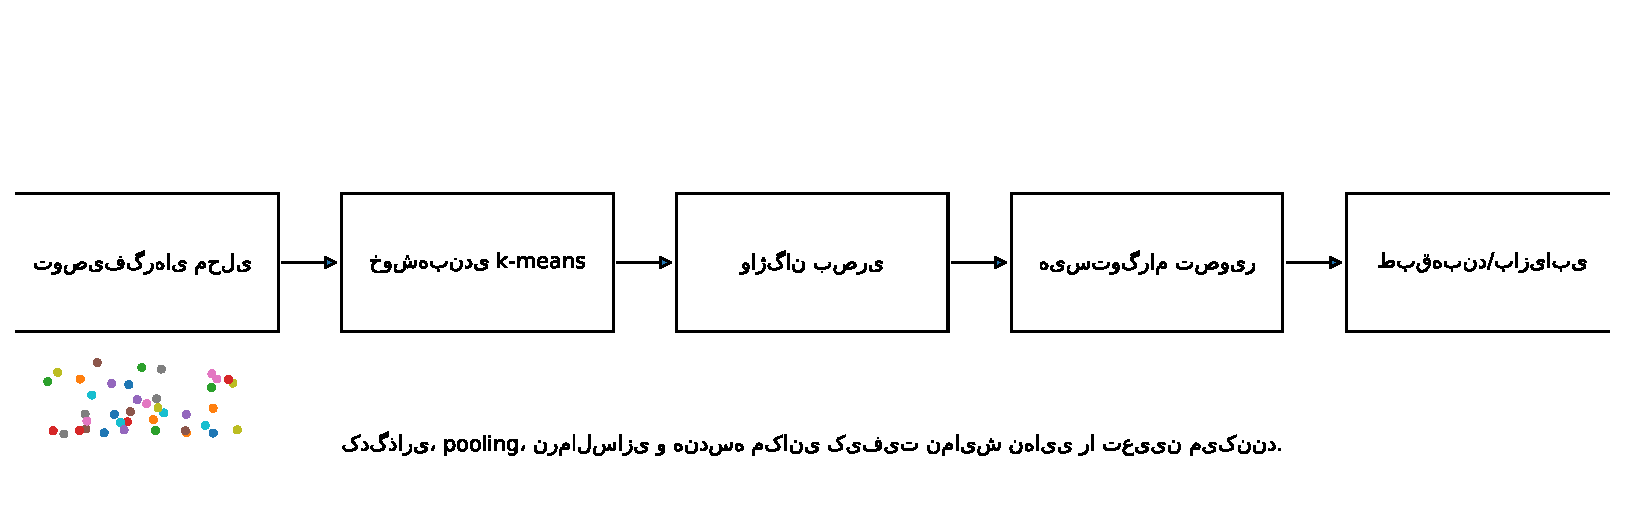
\includegraphics[width=0.97\textwidth]{fig09_09_bovw.pdf}
\caption{خط لوله BoVW. انتخاب descriptor، codebook، assignment، weighting و pooling همگی بخشی از مدل‌اند.}
\label{fig:bovw}
\end{figure}

\subsection{hard، soft و multiple assignment}
Hard assignment discontinuous است. در soft assignment:
\begin{equation}
w_{ik}=\frac{\exp(-\beta\norm{\vect d_i-\vect c_k}^2)}
{\sum_{\ell}\exp(-\beta\norm{\vect d_i-\vect c_\ell}^2)},
\qquad h_k=\sum_iw_{ik}.
\end{equation}
multiple assignment فقط چند centroid نزدیک را فعال می‌کند. soft assignment quantization error را کم، اما sparsity و سرعت inverted index را کاهش می‌دهد.

\subsection{TF--IDF و فهرست معکوس}
برای تصویر $j$ و واژه $k$:
\begin{equation}
\mathrm{tf}_{kj}=\frac{n_{kj}}{\sum_\ell n_{\ell j}},\qquad
\mathrm{idf}_k=\log\frac{N+1}{N_k+1},\qquad
v_{kj}=\mathrm{tf}_{kj}\mathrm{idf}_k.
\end{equation}
واژه‌ای که در همه تصاویر است قدرت تشخیص کمی دارد. inverted index برای هر واژه posting list تصاویر دارای آن را ذخیره و جست‌وجو را به اشتراک واژه‌ها محدود می‌کند؛ این ایده video Google و image retrieval کلاسیک را مقیاس‌پذیر کرد \cite{sivic2003,nister2006}.

\begin{figure}[H]
\centering
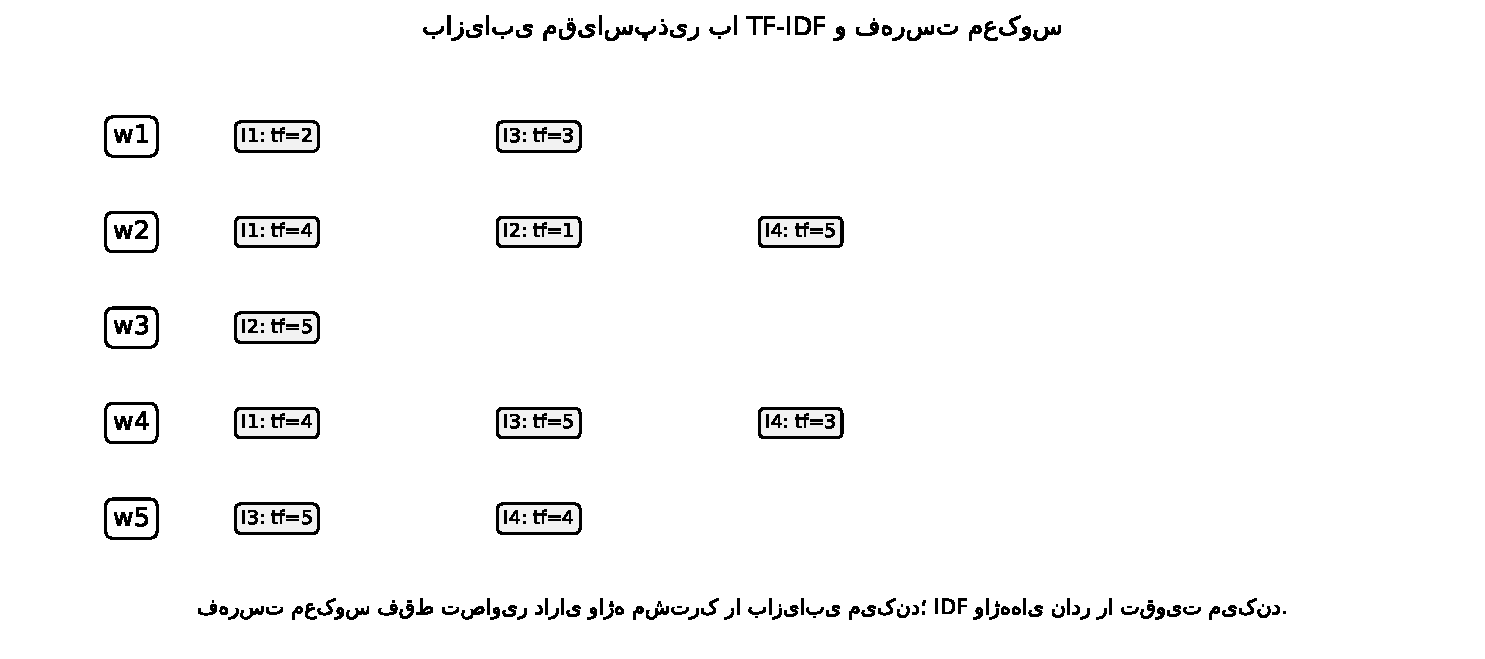
\includegraphics[width=0.88\textwidth]{fig09_13_inverted_index.pdf}
\caption{فهرست معکوس. واژه‌های query به posting listها می‌روند؛ TF--IDF و normalization score تصویر را می‌سازند.}
\label{fig:inverted}
\end{figure}

\subsection{burstiness و stop words}
بافت تکراری ممکن است یک واژه را ده‌ها بار در یک تصویر تکرار کند و score را مصنوعی بالا ببرد. راهکارها:
\begin{itemize}
\item power normalization $h_i\leftarrow\sign(h_i)|h_i|^\alpha$ با $0<\alpha<1$؛
\item capped term frequency؛
\item حذف visual stop wordهای بسیار رایج؛
\item geometric verification پس از retrieval اولیه.
\end{itemize}

\subsection{Spatial Pyramid Matching}
BoVW ترتیب مکانی را حذف می‌کند. Spatial Pyramid تصویر را در سطح $\ell$ به $2^\ell\times2^\ell$ سلول تقسیم و histogramهای سلولی را concat می‌کند:
\begin{equation}
\Phi(I)=\left[\sqrt{w_0}\vect h^{(0)},\sqrt{w_1}\vect h^{(1)},\ldots,\sqrt{w_L}\vect h^{(L)}\right].
\end{equation}
kernel histogram intersection weighted، تطابق ریزتر را بیشتر وزن می‌دهد \cite{lazebnik2006}.

\begin{figure}[H]
\centering
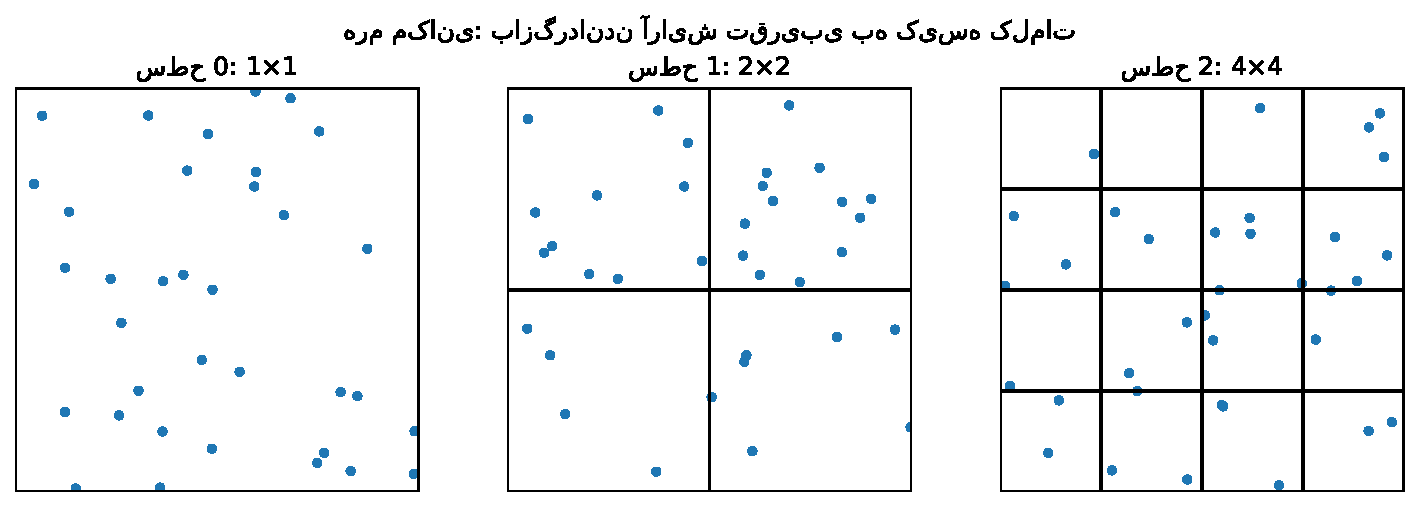
\includegraphics[width=0.92\textwidth]{fig09_10_spatial_pyramid.pdf}
\caption{هرم مکانی. نمایش به‌تدریج از orderless به حفظ آرایش تقریبی می‌رود، اما ابعاد با تعداد سلول‌ها رشد می‌کند.}
\label{fig:spm}
\end{figure}

\begin{algorithmbox}{الگوریتم 9.5 ـ آموزش BoVW بدون leakage}
\begin{enumerate}
\item split را در سطح شیء/ویدئو/فرد/صحنه انجام دهید.
\item descriptorها را فقط از train و با سقف نمونه در هر تصویر جمع کنید.
\item preprocessing مانند RootSIFT/PCA را فقط روی train برازش کنید.
\item k-means را با چند initialization آموزش و distortion را ثبت کنید.
\item train/validation/test را با codebook ثابت encode کنید.
\item weighting و normalization را داخل pipeline اعمال کنید.
\item classifier و hyperparameterها را روی validation انتخاب کنید.
\item test را یک بار ارزیابی و codebook hash و seed را ذخیره کنید.
\end{enumerate}
\end{algorithmbox}

\subsection{VLAD: تجمیع residual}
BoVW فقط count را نگه می‌دارد. VLAD برای هر centroid residual descriptorهای تخصیص‌یافته را جمع می‌کند:
\begin{equation}
\vect v_k=\sum_{i:a_i=k}(\vect d_i-\vect c_k),
\qquad \vect v=[\vect v_1;\ldots;\vect v_K].
\end{equation}
intra-normalization هر block و سپس power+$\ell_2$ normalization burstiness را کنترل می‌کند. VLAD اطلاعات مرتبه اول نسبت به codeword را حفظ می‌کند و برای retrieval/recognition قوی‌تر از count خام است \cite{jegou2010}.

\subsection{Fisher Vector: گرادیان log-likelihood}
فرض کنید descriptorها از GMM با پارامتر $\lambda=\{\pi_k,\mu_k,\sigma_k\}$ آمده‌اند. Fisher Vector گرادیان log-likelihood داده نسبت به پارامتر مدل است:
\begin{equation}
\mathcal G_\lambda(I)=\frac1N\nabla_\lambda\log p(\{\vect d_i\}\mid\lambda).
\end{equation}
برای covariance قطری و responsibility $\gamma_i(k)$، مؤلفه میانگین:
\begin{equation}
\vect u_k=\frac{1}{N\sqrt{\pi_k}}
\sum_i\gamma_i(k)\frac{\vect d_i-\vect\mu_k}{\vect\sigma_k},
\end{equation}
و مؤلفه واریانس:
\begin{equation}
\vect v_k=\frac{1}{N\sqrt{2\pi_k}}
\sum_i\gamma_i(k)
\left[\frac{(\vect d_i-\vect\mu_k)^2}{\vect\sigma_k^2}-1\right].
\end{equation}
FV آمار مرتبه اول و دوم را نسبت به مدل مولد ثبت می‌کند. power normalization و linear SVM بخش جدایی‌ناپذیر pipeline‌اند \cite{perronnin2010,sanchez2013}.

\begin{longtable}{p{24mm}p{31mm}p{29mm}p{29mm}p{25mm}}
\toprule
نمایش & اطلاعات نگه‌داشته & بعد تقریبی & مزیت & محدودیت \\
\midrule
BoVW & count واژه & $K$ & sparse، inverted index & quantization و حذف geometry \\
SPM & count در سلول & $K\sum4^\ell$ & ساختار مکانی & بعد زیاد، grid سخت \\
VLAD & residual مرتبه اول & $KD$ & compact و قوی & dense و حساس به normalization \\
FV & آمار مرتبه ۱ و ۲ GMM & $2KD$ & بیان غنی، linear classifier & حافظه و پیچیدگی بیشتر \\
\bottomrule
\end{longtable}

\section{بازشناسی کلاسیک شیء و چهره: خط لوله کامل}
\subsection{HOG + SVM برای آشکارسازی شیء}
در detector لغزان، برای هر window بردار HOG ساخته و score خطی
\begin{equation}
s(\vect x)=\vect w\trans\Phi_{\mathrm{HOG}}(\vect x)+b
\end{equation}
محاسبه می‌شود. pyramid تصویر scaleهای شیء را پوشش می‌دهد. پنجره‌های هم‌پوشان با non-maximum suppression ادغام می‌شوند. در NMS کلاسیک، box با score بالاتر انتخاب و boxهای با
\begin{equation}
\IoU(B_i,B_j)=\frac{|B_i\cap B_j|}{|B_i\cup B_j|}>\tau_{\mathrm{nms}}
\end{equation}
حذف می‌شوند. hard-negative mining نقش مهمی دارد: پس از آموزش اولیه، false positiveهای واقعی detector از تصاویر منفی جمع و مدل دوباره آموزش داده می‌شود.

\begin{algorithmbox}{الگوریتم 9.6 ـ HOG--SVM با hard-negative mining}
\begin{enumerate}
\item نمونه‌های مثبت را هم‌تراز و window استاندارد تعریف کنید.
\item از تصاویر منفی windowهای تصادفی اولیه بگیرید.
\item HOG را با cell، block، bin و normalization ثابت استخراج کنید.
\item linear SVM را آموزش دهید.
\item detector را روی تصاویر منفی کامل اجرا و false positiveهای پرامتیاز را جمع کنید.
\item مجموعه منفی را با hard negativeها گسترش و SVM را بازآموزی کنید.
\item روی validation threshold score و NMS را انتخاب کنید؛ test را دست‌نخورده نگه دارید.
\end{enumerate}
\end{algorithmbox}

\subsection{Deformable Part Model}
DPM شیء را با root filter و part filterهای جابه‌جاشونده مدل می‌کند:
\begin{equation}
S(\vect x,\vect z)=\sum_i\vect w_i\trans\Phi(I,\vect z_i)-
\sum_i\vect d_i\trans\psi(\Delta\vect z_i)+b.
\end{equation}
جمله deformation معمولاً شامل $[dx,dy,dx^2,dy^2]$ است. inference با distance transform سریع و آموزش با latent SVM انجام می‌شود. اهمیت تاریخی DPM در formalization
«appearance + geometry + latent parts» است؛ ایده‌ای که در مدل‌های مدرن نیز بازمی‌گردد \cite{felzenszwalb2010}.

\subsection{Eigenfaces، Fisherfaces و زیر‌فضاهای چهره}
برای چهره، alignment از خود classifier مهم‌تر است. crop، scale، landmark و نور باید قرارداد ثابتی داشته باشند. pipeline کلاسیک:
\[
\text{detect}\to\text{align}\to\text{photometric normalize}\to\text{PCA/LDA}\to\text{distance/classifier}.
\]
در open-set recognition، threshold فاصله برای رد هویت ناشناخته لازم است. accuracy closed-set بدون گزارش false accept/false reject برای کاربرد امنیتی کافی نیست.

\subsection{Local Binary Pattern Histogram}
LBP برای پیکسل مرکز $g_c$ و همسایه‌ها $g_p$:
\begin{equation}
\mathrm{LBP}_{P,R}=\sum_{p=0}^{P-1}s(g_p-g_c)2^p,
\qquad s(z)=\mathbf1[z\ge0].
\end{equation}
Histogram LBP در grid مکانی برای texture و چهره استفاده می‌شود. چون فقط ترتیب intensity را می‌گیرد، نسبت به تغییر monotonic روشنایی مقاوم است؛ اما نویز نزدیک threshold بیت‌ها را ناپایدار می‌کند. الگوهای uniform تعداد transitionهای ۰/۱ کم دارند و ابعاد را کاهش می‌دهند.

\section{یادگیری متریک و بازشناسی مبتنی بر فاصله}
گاهی classifier ثابت کافی نیست و می‌خواهیم فاصله، شباهت معنایی یا هویتی را بازتاب دهد. Mahalanobis metric
\begin{equation}
d_M^2(\vect x_i,\vect x_j)=(\vect x_i-\vect x_j)\trans\mat M(\vect x_i-\vect x_j),\qquad \mat M\succeq0
\end{equation}
با $\mat M=\mat L\trans\mat L$ معادل Euclidean بعد از projection است. یک objective ساده pairwise:
\begin{equation}
\min_{\mat M\succeq0}
\sum_{(i,j)\in\mathcal S}d_M^2(\vect x_i,\vect x_j)
+\lambda\sum_{(i,j)\in\mathcal D}[m-d_M^2(\vect x_i,\vect x_j)]_+.
\end{equation}
LMNN همسایه‌های هدف را نزدیک و impostorها را بیرون حاشیه نگه می‌دارد. این بخش پل مفهومی به contrastive/triplet loss است، اما در خط لوله کلاسیک می‌توان $M$ را با optimization محدب آموخت.

\section{تطبیق چندتصویری، مسیر و مکان}
ویژگی و تطبیق تنها برای دو تصویر نیستند. در panorama، SfM، SLAM و visual localization، graph مشاهده ساخته می‌شود:
\begin{equation}
\mathcal G=(\mathcal V_{\mathrm{images}}\cup\mathcal V_{\mathrm{tracks}},\mathcal E_{\mathrm{obs}}).
\end{equation}
یک track مجموعه keypointهایی است که یک نقطه سه‌بعدی را در چند تصویر می‌بینند. union کور pairwise matchها می‌تواند inconsistency بسازد؛ cycle consistency باید بررسی شود. اگر $i\leftrightarrow j$ و $j\leftrightarrow k$، correspondence $i\leftrightarrow k$ باید با geometry سازگار باشد.

\subsection{retrieval سپس localization}
برای پایگاه بزرگ، ابتدا global descriptor یا BoVW چند تصویر نامزد را بازیابی می‌کند؛ سپس local matching و PnP روی هر نامزد اجرا می‌شود. این طراحی coarse-to-fine هزینه را کاهش می‌دهد:
\[
\text{global retrieval}\rightarrow\text{local matching}\rightarrow\text{2D--3D PnP}\rightarrow\text{pose refinement}.
\]
در سیستم حرفه‌ای، recall@K retrieval و pose accuracy جدا گزارش می‌شوند تا معلوم شود شکست از بازیابی است یا هندسه.

\section{روش‌های آموختنی: ادامه یا جایگزین خط لوله کلاسیک؟}
روش‌های آموختنی سه الگو دارند:
\begin{enumerate}
\item detector و descriptor را می‌آموزند، اما matching و RANSAC کلاسیک می‌ماند؛
\item matcher، context و assignment را می‌آموزد، ولی keypoint خارجی می‌گیرد؛
\item detector-free یا dense matching correspondence را مستقیماً از دو تصویر می‌سازد.
\end{enumerate}

\subsection{SuperPoint: آشکارسازی و توصیف self-supervised}
SuperPoint یک encoder مشترک و دو head detector/descriptor دارد. ابتدا detector مصنوعی روی شکل‌های هندسی آموزش و با Homographic Adaptation روی تصاویر واقعی self-label تولید می‌شود. descriptor با correspondenceهای ناشی از homography آموزش می‌بیند \cite{detone2018}. مزیت آن co-design detector و descriptor است؛ محدودیت آن وابستگی به distribution آموزش و مدل transformation self-supervision است.

\subsection{SuperGlue و LightGlue}
SuperGlue مجموعه keypointها و descriptorها را با self/cross-attention contextualize و assignment را با optimal transport differentiable حل می‌کند \cite{sarlin2020}. LightGlue طراحی سبک‌تر با confidence، early stopping و point pruning ارائه می‌کند؛ برای pairهای آسان عمق کمتری مصرف می‌کند و matching sparse را کاراتر می‌سازد \cite{lindenberger2023}.

\subsection{LoFTR و detector-free matching}
LoFTR به‌جای آشکارسازی مستقل، feature mapهای دو تصویر را با transformer مرتبط و coarse-to-fine match می‌کند. این روش در ناحیه کم‌بافت یا تکرارپذیری ضعیف keypoint مزیت دارد، اما correspondenceهای متراکم‌تر، حافظه و filtering متفاوت می‌طلبند \cite{sun2021}. Efficient LoFTR در ۲۰۲۴ هدف کاهش هزینه و نزدیک‌شدن سرعت به روش sparse را دنبال کرد \cite{wang2024loftr}.

\subsection{Dense matching و ویژگی‌های بنیادی}
RoMa از featureهای pretrained DINOv2 برای dense matching robust بهره می‌گیرد و confidence/warp را پیش‌بینی می‌کند \cite{edstedt2024}. OmniGlue ترکیب featureهای foundation با keypoint matcher را برای generalization مطرح می‌کند \cite{jiang2024}. RDD در CVPR 2025 detector و descriptor مبتنی بر deformable transformer را برای تغییر دید و مقیاس شدید ارائه کرد \cite{chen2025rdd}. در CVPR 2026 نیز تطبیق‌گرهای مبتنی بر state-space و sparse correlation به مقیاس‌پذیری pairهای بزرگ‌تر پرداخته‌اند \cite{choo2026}.

\begin{figure}[H]
\centering
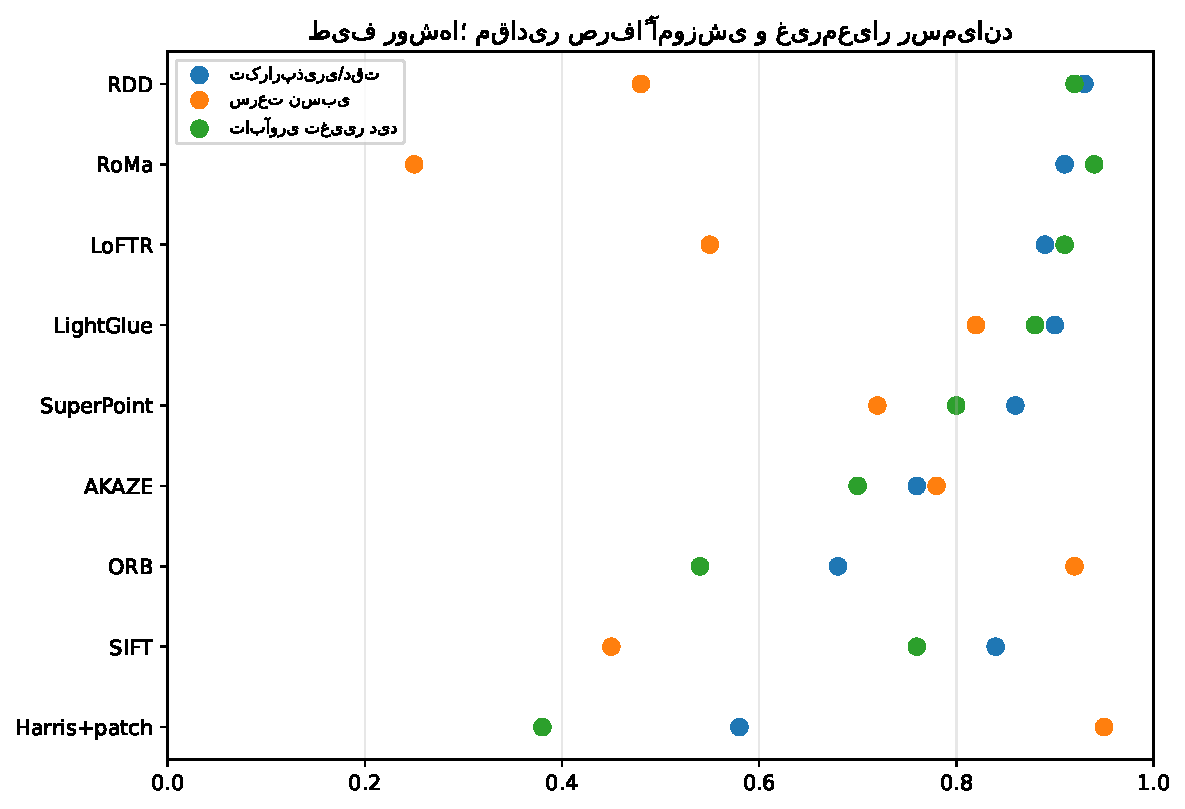
\includegraphics[width=0.82\textwidth]{fig09_15_classic_modern.pdf}
\caption{نمای آموزشی طیف کلاسیک تا آموختنی. نقاط شکل benchmark رسمی نیستند؛ هدف نمایش trade-off میان سرعت، robustness و complexity است.}
\label{fig:classicmodern}
\end{figure}

\begin{futurebox}
دهه آینده احتمالاً «یک matcher واحد برای همه» نخواهد داشت. سیستم‌های واقعی از ترکیب زیر سود می‌برند:
\begin{itemize}
\item descriptor کلاسیک برای latency کم، CPU و explainability؛
\item feature آموختنی برای تغییر viewpoint، illumination و texture-poor؛
\item هندسه کلاسیک برای تضمین سازگاری فیزیکی؛
\item uncertainty و failure detection برای جلوگیری از اعتماد کور؛
\item retrieval foundation-based و verification local برای مقیاس بزرگ.
\end{itemize}
\end{futurebox}

\begin{researchbox}[مقایسه منصفانه کلاسیک و آموختنی]
تعداد match خام را مقایسه نکنید. برای هر روش، detector budget، resolution، preprocessing، matcher، geometric model، threshold residual و compute device را ثبت کنید. معیارها باید شامل
precision match، recall correspondence، تعداد inlier، pose AUC، failure rate، latency و memory باشند. استفاده RANSAC متفاوت می‌تواند نتیجه feature را وارونه کند.
\end{researchbox}

\section{ارزیابی آشکارساز و تطبیق‌گر}
\subsection{repeatability}
اگر $N_1,N_2$ تعداد نواحی قابل مشاهده و $N_{\mathrm{rep}}$ زوج تکرارشده باشد:
\begin{equation}
\mathrm{repeatability}=\frac{N_{\mathrm{rep}}}{\min(N_1,N_2)}.
\end{equation}
تعریف visibility، overlap threshold و correspondence یک‌به‌یک باید صریح باشد. repeatability بالا بدون descriptor discriminative matching خوب را تضمین نمی‌کند.

\subsection{matching precision، recall و score}
اگر $M$ match پذیرفته، $C$ صحیح و $G$ correspondence قابل مشاهده باشد:
\begin{equation}
\mathrm{precision}=\frac{C}{M},\qquad
\mathrm{recall}=\frac{C}{G}.
\end{equation}
آستانه ratio یا confidence منحنی PR می‌سازد. AP area زیر PR است و در class imbalance مناسب‌تر از ROC می‌تواند باشد.

\begin{figure}[H]
\centering
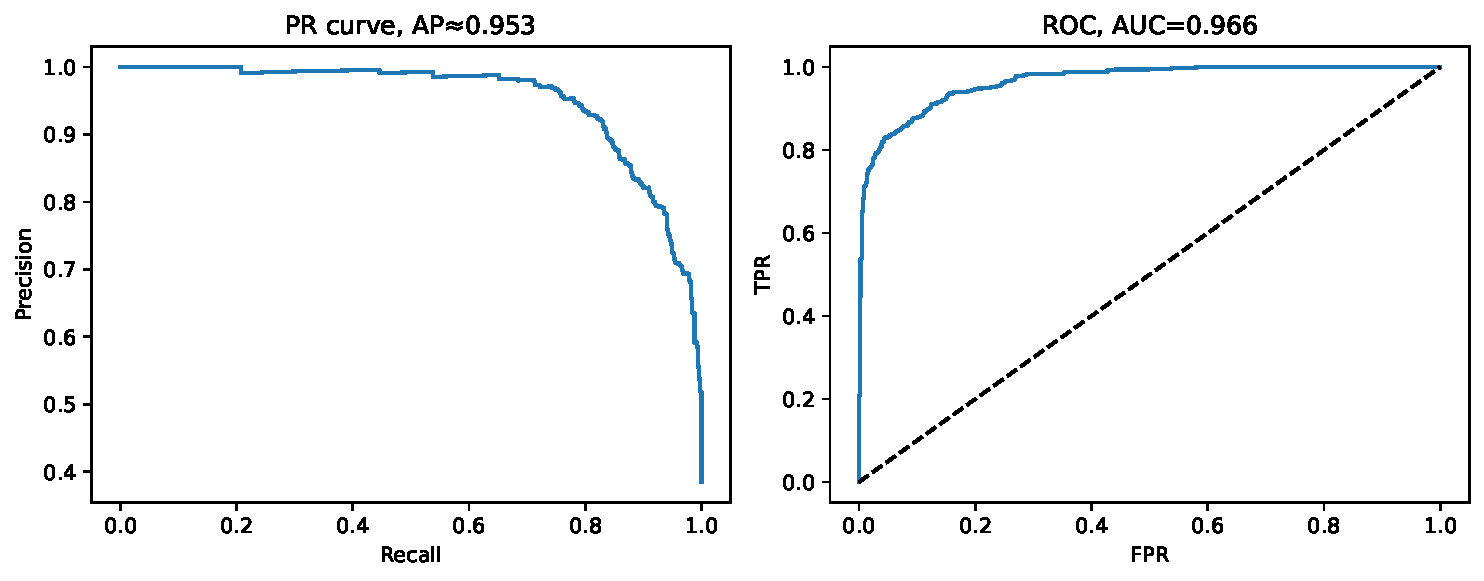
\includegraphics[width=0.92\textwidth]{fig09_14_metrics.pdf}
\caption{آستانه matcher نقطه operating را روی PR/ROC انتخاب می‌کند. یک عدد accuracy رفتار threshold را پنهان می‌کند.}
\label{fig:prroc}
\end{figure}

\subsection{خطای هندسی و pose AUC}
برای homography، corner reprojection؛ برای relative pose، خطای دوران و جهت انتقال:
\begin{align}
e_R&=\arccos\left(\frac{\trace(\mat R_{\mathrm{gt}}\mat R_{\mathrm{est}}\trans)-1}{2}\right),\\
e_t&=\arccos\left(\frac{\vect t_{\mathrm{gt}}\trans\vect t_{\mathrm{est}}}{\norm{\vect t_{\mathrm{gt}}}\norm{\vect t_{\mathrm{est}}}}\right).
\end{align}
معمولاً $e=\max(e_R,e_t)$ و AUC تا thresholdهایی مانند ۵، ۱۰ و ۲۰ درجه گزارش می‌شود. median فقط شکست‌های کامل را پنهان می‌کند؛ failure rate نیز لازم است.

\subsection{ارزیابی بازشناسی}
برای confusion matrix $C_{ij}$، macro average به هر کلاس وزن برابر و micro average به هر نمونه وزن برابر می‌دهد. در عدم توازن، accuracy ممکن است گمراه‌کننده باشد. برای retrieval:
\begin{equation}
\AP(q)=\frac{1}{N_q^+}\sum_{k=1}^N P_q(k)\,\mathrm{rel}_q(k),
\qquad \mAP=\frac1Q\sum_q\AP(q).
\end{equation}
در instance retrieval باید distractorها، query crop، multi-scale و geometric re-ranking تعریف شوند.

\subsection{پروتکل robustness}
تغییرات را جدا و ترکیبی بسنجید:
\begin{itemize}
\item blur، noise، JPEG، gamma و exposure؛
\item rotation، scale، affine viewpoint و perspective؛
\item seasonal/day-night، modality RGB--IR، underwater یا medical؛
\item occlusion، dynamic objects و repetitive texture؛
\item rolling shutter و motion blur؛
\item کمبود texture و saturation.
\end{itemize}
گزارش average روی همه corruptionها کافی نیست؛ failure taxonomy و بدترین گروه کاربردی مهم‌اند.

\begin{longtable}{p{33mm}p{49mm}p{55mm}}
\toprule
لایه ارزیابی & معیار & نکته گزارش \\
\midrule
آشکارسازی & repeatability، localization، coverage & budget و visibility ثابت \\
توصیف/تطبیق & PR، AP، matching score & metric و ratio threshold ثابت \\
هندسه & inlier ratio، reprojection، pose AUC & RANSAC و مدل یکسان \\
بازیابی & Recall@K، mAP، query time & distractor scale و index memory \\
بازشناسی & macro-F1، balanced accuracy، ROC/PR & split گروهی و calibration \\
مهندسی & latency، throughput، memory، energy & CPU/GPU، batch=1 و warm-up \\
پایداری & corruption/OOD/failure rate & گروه‌بندی و فاصله اطمینان \\
\bottomrule
\end{longtable}

\section{آزمایشگاه کدنویسی فصل}
\subsection{Harris از صفر با قرارداد نوع داده}
\begin{latin}
\begin{lstlisting}
from __future__ import annotations
import numpy as np
from scipy.ndimage import gaussian_filter, maximum_filter

def harris_response(
    image: np.ndarray,
    sigma_d: float = 1.0,
    sigma_i: float = 2.0,
    k: float = 0.04,
) -> np.ndarray:
    """Compute Harris response on a 2-D image scaled to [0, 1]."""
    if image.ndim != 2:
        raise ValueError("image must be grayscale")
    x = image.astype(np.float64)
    if not np.isfinite(x).all():
        raise ValueError("image contains NaN/Inf")
    x = (x - x.min()) / (x.max() - x.min() + 1e-12)
    smooth = gaussian_filter(x, sigma_d)
    iy, ix = np.gradient(smooth)
    sxx = gaussian_filter(ix * ix, sigma_i)
    syy = gaussian_filter(iy * iy, sigma_i)
    sxy = gaussian_filter(ix * iy, sigma_i)
    det = sxx * syy - sxy * sxy
    trace = sxx + syy
    return det - k * trace * trace

def select_keypoints(response: np.ndarray, n: int = 1000, radius: int = 4):
    local_max = response == maximum_filter(response, size=2 * radius + 1)
    values = response[local_max]
    coords = np.argwhere(local_max)
    keep = np.argsort(values)[::-1][:n]
    return coords[keep], values[keep]
\end{lstlisting}
\end{latin}
آزمایش property-based: با افزودن ثابت روشنایی پاسخ gradient تغییر نکند؛ با ضرب intensity پاسخ Harris به توان چهار scale شود؛ مختصات تحت translation داخلی همان translation را دنبال کند.

\subsection{RANSAC خط و تعمیم به homography}
\begin{latin}
\begin{lstlisting}
from dataclasses import dataclass
import numpy as np

@dataclass
class RansacResult:
    model: tuple[float, float]
    inliers: np.ndarray
    residuals: np.ndarray

def ransac_line(xy: np.ndarray, threshold: float, max_trials: int = 2000,
                confidence: float = 0.999, seed: int = 0) -> RansacResult:
    rng = np.random.default_rng(seed)
    n = len(xy)
    if n < 2:
        raise ValueError("at least two points are required")
    best_mask = np.zeros(n, dtype=bool)
    best_model = (0.0, 0.0)
    trials = 0
    target_trials = max_trials
    while trials < min(max_trials, target_trials):
        i, j = rng.choice(n, size=2, replace=False)
        dx = xy[j, 0] - xy[i, 0]
        if abs(dx) < 1e-12:
            trials += 1
            continue
        a = (xy[j, 1] - xy[i, 1]) / dx
        b = xy[i, 1] - a * xy[i, 0]
        residuals = np.abs(a * xy[:, 0] - xy[:, 1] + b) / np.sqrt(a*a + 1)
        mask = residuals < threshold
        if mask.sum() > best_mask.sum():
            best_mask = mask
            best_model = (a, b)
            w = max(mask.mean(), 1e-12)
            p_good = max(1.0 - w**2, 1e-12)
            target_trials = int(np.ceil(np.log(1-confidence) / np.log(p_good)))
        trials += 1
    a, b = np.polyfit(xy[best_mask, 0], xy[best_mask, 1], 1)
    residuals = np.abs(a * xy[:, 0] - xy[:, 1] + b) / np.sqrt(a*a + 1)
    return RansacResult((float(a), float(b)), residuals < threshold, residuals)
\end{lstlisting}
\end{latin}
برای homography، minimal solver چهار correspondence نرمال‌شده DLT است؛ residual را symmetric transfer بگیرید و sampleهای با مساحت کم را پیش از solve رد کنید.

\subsection{BoVW + SVM در pipeline امن}
\begin{latin}
\begin{lstlisting}
from sklearn.cluster import MiniBatchKMeans
from sklearn.preprocessing import normalize
from sklearn.svm import LinearSVC
import numpy as np

def fit_codebook(train_descriptors: list[np.ndarray], k: int, seed: int = 0):
    pool = np.concatenate([d for d in train_descriptors if d is not None], axis=0)
    km = MiniBatchKMeans(n_clusters=k, batch_size=4096, random_state=seed,
                         n_init=10, reassignment_ratio=0.01)
    km.fit(pool)
    return km

def encode_bovw(descriptors: list[np.ndarray], codebook) -> np.ndarray:
    features = np.zeros((len(descriptors), codebook.n_clusters), dtype=np.float64)
    for i, d in enumerate(descriptors):
        if d is None or len(d) == 0:
            continue
        words = codebook.predict(d)
        features[i] = np.bincount(words, minlength=codebook.n_clusters)
    features = np.sqrt(features)  # power normalization for counts
    return normalize(features, norm="l2")

# IMPORTANT: descriptors_test never participate in codebook fitting.
codebook = fit_codebook(descriptors_train, k=512, seed=42)
Xtr = encode_bovw(descriptors_train, codebook)
Xva = encode_bovw(descriptors_val, codebook)
model = LinearSVC(C=1.0, class_weight="balanced").fit(Xtr, y_train)
\end{lstlisting}
\end{latin}

\begin{codecontract}
هر آزمایش باید چهار جدول جدا بسازد: detector statistics، descriptor/matching statistics، geometry statistics و task statistics. ادغام همه چیز در accuracy نهایی، محل شکست را پنهان می‌کند. همه arrayها، thresholdها و random seedها باید ذخیره شوند.
\end{codecontract}

\section{طراحی آزمایش‌های عمیق و بازتولیدپذیر}
\subsection{آزمایش ۱: ناوردایی کنترل‌شده}
یک تصویر مرجع و transformation grid بسازید:
\[
\theta\in[-90^\circ,90^\circ],\quad s\in[0.5,2],\quad
\text{blur}\in[0,4],\quad \gamma\in[0.5,2],\quad \text{noise}\in[0,0.1].
\]
برای Harris+patch، SIFT، ORB و AKAZE repeatability، match precision و homography error را رسم کنید. هر transformation را تنها و سپس دو‌به‌دو اعمال کنید تا interaction دیده شود.

\subsection{آزمایش ۲: threshold و trade-off}
برای ratio $\rho$ از ۰٫۵ تا ۱، PR curve و RANSAC runtime را ثبت کنید. ratio سخت precision را بالا می‌برد، اما ممکن است inlier کافی برای minimal model باقی نگذارد. operating point باید با success pose، نه فقط descriptor precision، انتخاب شود.

\subsection{آزمایش ۳: descriptor budget}
تعداد keypoint را $250,500,1000,2000,4000$ تغییر دهید. زمان detect، describe، match و RANSAC، memory و pose AUC را گزارش کنید. curve saturation نشان می‌دهد نقطه بیشتر چه زمانی فقط هزینه و ambiguity می‌افزاید.

\subsection{آزمایش ۴: BoVW، VLAD و FV}
با descriptor ثابت، codebook size و PCA dimension را تغییر دهید. برای هر representation، power normalization، $\ell_2$ و classifier ثابت را مقایسه کنید. train codebook time، feature dimension، disk size، inference و macro-F1/mAP گزارش شود.

\subsection{آزمایش ۵: کلاسیک در برابر آموختنی}
SIFT+ratio+MAGSAC++، SuperPoint+LightGlue، Efficient LoFTR و یک dense matcher را روی subsetهای viewpoint، illumination و texture-poor اجرا کنید. resolution و geometric verifier را تا حد ممکن یکسان کنید. علاوه بر average، بدترین decile و failure rate را گزارش کنید.

\subsection{آزمایش ۶: domain shift}
مدل یا threshold را روی indoor/day تنظیم و روی outdoor/night، RGB--IR یا تصاویر صنعتی آزمون کنید. روش کلاسیک نیز hyperparameter دارد؛ ادعای «بدون آموزش» به معنی «بدون تنظیم» نیست.

\section{خطاهای رایج در مقاله و پروژه}
\begin{enumerate}
\item نمایش چند خط match رنگی و نتیجه‌گیری کیفی بدون ground truth.
\item گزارش تعداد match خام به‌جای inlier هندسی و pose accuracy.
\item استفاده matcher یا metric ناسازگار با descriptor.
\item تنظیم ratio/RANSAC روی test.
\item ساخت codebook، PCA یا normalization statistics روی کل داده.
\item split تصادفی frameهای یک ویدئو در train و test.
\item مقایسه SIFT در resolution کامل با مدل عمیق در resolution کوچک یا بالعکس.
\item نادیده‌گرفتن latency feature extraction و فقط گزارش matcher.
\item استفاده homography برای صحنه سه‌بعدی عمومی و تفسیر inlier زیاد به‌عنوان درستی pose.
\item حذف pairهای شکست‌خورده از میانگین.
\item گزارش تنها accuracy در open-set recognition.
\item استفاده تصویر نمونه مشهور و عدم ارزیابی روی dataset واقعی دامنه هدف.
\end{enumerate}

\section{پرسش‌های تصمیم مهندسی}
\begin{longtable}{p{48mm}p{91mm}}
\toprule
پرسش & پاسخ طراحی \\
\midrule
CPU و latency سخت؟ & ORB/AKAZE، Hamming، grid coverage و geometry کلاسیک را baseline کنید. \\
تغییر دید و نور شدید؟ & SIFT/RootSIFT یا feature آموختنی؛ affine/dense matcher و verifier robust. \\
بافت کم؟ & detector-free/dense matching یا line/region feature؛ keypoint صرف ممکن است پوشش ندهد. \\
پایگاه میلیون‌تصویری؟ & global/coarse retrieval، inverted index/PQ، سپس local verification. \\
نیاز به توضیح و certification؟ & residual، inlier mask، geometry، uncertainty و fallback کلاسیک حفظ شود. \\
دامنه خاص و داده کم؟ & classical strong baseline + adaptation سبک؛ از fine-tune بزرگ بدون validation پرهیز. \\
چهره/هویت open-set؟ & metric، threshold rejection، ROC/FAR/FRR و group-aware split. \\
قطعه صنعتی ثابت؟ & template/edge/chamfer ممکن است از شبکه پیچیده مناسب‌تر و قابل ممیزی‌تر باشد. \\
\bottomrule
\end{longtable}

\section{تمرین‌های نظری و اثباتی}
\begin{enumerate}
\item ناوردایی ZNCC نسبت به $I'=aI+b$ برای $a>0$ را اثبات کنید و حالت $a<0$ را تحلیل کنید.
\item معادله تانسور ساختار \eqref{eq:structure_tensor_feature} را از تیلور استخراج کنید.
\item نواحی تصمیم Harris را در صفحه $(\lambda_1,\lambda_2)$ برای چند $k$ رسم کنید.
\item نشان دهید مقیاس پاسخ Harris با ضرب intensity چگونه تغییر می‌کند.
\item رابطه DoG و LoG را با بسط تیلور نسبت به $\sigma$ استخراج کنید.
\item برای Gaussian blob دوبعدی، مقیاس اکسترمم $\sigma^2\nabla^2L$ را محاسبه کنید.
\item معادله offset زیرپیکسلی \eqref{eq:subpixel} را از شرط ایستایی به دست آورید.
\item رابطه edge rejection در SIFT را برحسب نسبت eigenvalue اثبات کنید.
\item نشان دهید برای بردارهای واحد، ranking فاصله Euclidean و cosine یکسان است.
\item یک distribution بسازید که ratio test بهتر از threshold مطلق عمل کند و یک مثال عکس آن ارائه دهید.
\item فرمول iteration RANSAC را استخراج و برای $w=0.3$ و مدل‌های ۲، ۴، ۵ و ۸ نقطه‌ای محاسبه کنید.
\item اثر overestimated و underestimated threshold RANSAC را بر bias و variance تحلیل کنید.
\item شرط تباهی چهار نقطه DLT homography را با rank matrix بیان کنید.
\item دوگان SVM را از Lagrangian primal استخراج کنید.
\item نشان دهید PCA label-invariant است و مثال دوکلاسی بسازید که مؤلفه اول برای طبقه‌بندی نامناسب باشد.
\item generalized eigenproblem LDA را از Rayleigh quotient استخراج کنید.
\item نشان دهید TF--IDF چگونه واژه موجود در همه تصاویر را کم‌وزن می‌کند.
\item ابعاد SPM، VLAD و FV را برای $K=256,D=64,L=2$ محاسبه کنید.
\item gradient log-likelihood GMM نسبت به $\mu_k$ را استخراج و فرمول FV mean را توجیه کنید.
\item رابطه precision/recall matcher و success probability RANSAC را به‌صورت تحلیلی بحث کنید.
\end{enumerate}

\section{پروژه‌های پایان فصل}
\subsection{پروژه A: آزمایشگاه ویژگی کلاسیک}
Harris، Shi--Tomasi، FAST، DoG و Hessian را با API مشترک بسازید. repeatability، localization، coverage و runtime را روی transformationهای کنترل‌شده مقایسه کنید.

\subsection{پروژه B: موتور تطبیق و panorama}
SIFT/ORB/AKAZE، ratio، mutual، RANSAC/MAGSAC++، homography و blending را پیاده‌سازی کنید. failure ناشی از parallax، motion و texture repetition را طبقه‌بندی کنید.

\subsection{پروژه C: بازشناسی کلاسیک کامل}
روی یک dataset چندکلاسه، HOG+SVM، LBP+SVM، BoVW، SPM، VLAD و FV را با split گروهی مقایسه کنید. ابعاد، زمان، حافظه، macro-F1 و calibration را گزارش کنید.

\subsection{پروژه D: بازیابی تصویر مقیاس‌پذیر}
TF--IDF، inverted index، stop-word، burstiness و geometric re-ranking را بسازید. Recall@K، mAP، query latency و index size را در اندازه پایگاه افزاینده اندازه‌گیری کنید.

\subsection{پروژه E: کلاسیک در برابر LightGlue/LoFTR}
روی HPatches یا یک مجموعه دامنه‌خاص، SIFT+MAGSAC++، SuperPoint+LightGlue و LoFTR را در پروتکل ثابت مقایسه کنید. نتیجه را به viewpoint، illumination و texture تقسیم کنید.

\subsection{پروژه F: open-set چهره یا شیء}
PCA/LDA/metric را با gallery/probe مستقل بسازید. CMC، ROC، FAR/FRR و rejection ناشناخته را گزارش و leakage هویت را کنترل کنید.

\section{پرامپت پیشنهادی برای Codex}
\begin{latin}
\begin{lstlisting}[language={}]
Build a fully reproducible Python research package for Chapter 9,
"Local Features, Matching, and Classical Recognition".

Implement from scratch where educationally useful:
- ZNCC and FFT phase correlation;
- Harris/Shi-Tomasi with subpixel localization and ANMS;
- Gaussian/DoG scale space, 3-D extrema, contrast and edge rejection;
- a compact educational SIFT-like descriptor with trilinear voting;
- BRIEF-style binary tests and Hamming matching;
- brute-force 2-NN, ratio test, mutual check and assignment diagnostics;
- adaptive RANSAC for line, homography and fundamental matrix, including
  degeneracy tests, normalized solvers and nonlinear refinement;
- detector repeatability, overlap error, matching PR/AP, reprojection error,
  relative-pose AUC and failure rate;
- BoVW, TF-IDF, inverted index, spatial pyramid, VLAD and Fisher Vector;
- PCA, LDA, kNN, linear/RBF SVM, calibrated scores and AdaBoost;
- HOG + sliding-window detection with hard-negative mining and NMS.

Use trusted library wrappers for SIFT, ORB, AKAZE, MAGSAC++, SuperPoint,
LightGlue, Efficient LoFTR, RoMa or other learned methods when licenses and
weights are available. Never silently download weights. Record checkpoint,
commit, license, image resolution, device and preprocessing.

Research protocol:
1. Use analytic synthetic transformations plus public benchmarks and one
   domain-specific dataset.
2. Split by object/scene/person/video before any PCA, codebook, whitening or
   hyperparameter fitting.
3. Compare methods at fixed keypoint budgets and fixed geometric verification.
4. Sweep ratio/confidence and RANSAC thresholds; produce PR and pose-success
   curves, not one cherry-picked operating point.
5. Log detect, describe, match, verify and end-to-end latency separately.
6. Save keypoints, descriptors metadata, matches, inlier masks, model matrices,
   residuals, seeds, configs, environment and data hashes.
7. Add robustness tests for scale, rotation, affine viewpoint, blur, noise,
   exposure, gamma, JPEG, occlusion, repeated texture and low texture.
8. Report paired bootstrap confidence intervals over independent image pairs
   or queries and preserve all failed pairs in the denominator.
9. Add unit/property tests for coordinate order, dtype/range, empty descriptors,
   Hamming vs L2 selection, normalized DLT, RANSAC degeneracy, deterministic
   sampling, label leakage and metric edge cases.
10. Provide a single command that regenerates every figure, CSV and table used
    by the chapter, plus an automatic failure gallery sorted by declared error.
\end{lstlisting}
\end{latin}

\section{تقسیم پیشنهادی ویدئوهای ۱۵ دقیقه‌ای}
\begin{longtable}{p{12mm}p{116mm}}
\toprule
بخش & موضوع \\
\midrule
1 & مسئله ویژگی، تطبیق و بازشناسی \\
2 & هم‌وردایی و ناوردایی با گروه تبدیل \\
3 & معیارهای repeatability، localization و coverage \\
4 & SSD و مدل نویز گاوسی \\
5 & SAD، NCC و ZNCC \\
6 & تصویر انتگرالی و تطبیق سریع \\
7 & phase correlation و قضیه شیفت فوریه \\
8 & انرژی تغییر وصله و Moravec \\
9 & استخراج تانسور ساختار \\
10 & Harris و صفحه مقادیر ویژه \\
11 & Shi--Tomasi و ANMS \\
12 & FAST، AGAST و درخت تصمیم \\
13 & ضرورت فضای مقیاس \\
14 & axioms فضای مقیاس گاوسی \\
15 & مشتق نرمال‌شده و LoG \\
16 & استخراج DoG از معادله گرما \\
17 & اکسترمم سه‌بعدی مکان--مقیاس \\
18 & مکان‌یابی زیرپیکسلی \\
19 & حذف کنتراست پایین و پاسخ لبه \\
20 & Hessian، SURF و blob \\
21 & KAZE/AKAZE و diffusion غیرخطی \\
22 & MSER و ناحیه maximally stable \\
23 & affine covariant region \\
24 & جهت‌گذاری canonical \\
25 & descriptor وصله خام و whitening \\
26 & ساخت SIFT مرحله‌به‌مرحله \\
27 & interpolation و نرمال‌سازی SIFT \\
28 & RootSIFT و فاصله Hellinger \\
29 & HOG و block normalization \\
30 & Shape Context و تطبیق contour \\
31 & BRIEF و آزمون‌های دودویی \\
32 & ORB، BRISK، FREAK و AKAZE \\
33 & فاصله L2، cosine، Mahalanobis و Hamming \\
34 & nearest neighbor و curse of dimensionality \\
35 & ratio test و تحلیل آماری آن \\
36 & mutual check و assignment \\
37 & FLANN، LSH و product quantization \\
38 & residual هندسی و انتخاب مدل \\
39 & استخراج احتمال iteration RANSAC \\
40 & threshold، uncertainty و فاصله Mahalanobis \\
41 & PROSAC، LO-RANSAC، USAC و MAGSAC++ \\
42 & degeneracy و model selection \\
43 & template/chamfer/generalized Hough \\
44 & ممان‌ها و descriptorهای کلی شکل \\
45 & PCA و Eigenfaces \\
46 & LDA و Fisherfaces \\
47 & kNN، LDA/QDA classifier \\
48 & SVM primal، margin و dual \\
49 & kernel، چندکلاسه و calibration \\
50 & AdaBoost، Haar و cascade \\
51 & HOG+SVM و hard-negative mining \\
52 & DPM و latent parts \\
53 & Bag of Visual Words و k-means \\
54 & hard/soft assignment و quantization \\
55 & TF--IDF و فهرست معکوس \\
56 & burstiness و stop words \\
57 & Spatial Pyramid Matching \\
58 & VLAD و residual aggregation \\
59 & Fisher Vector و gradient GMM \\
60 & retrieval سپس geometric verification \\
61 & track، cycle consistency و چندتصویری \\
62 & SuperPoint و self-supervision هندسی \\
63 & SuperGlue و assignment آموختنی \\
64 & LightGlue و تطبیق تطبیقی سریع \\
65 & LoFTR و detector-free matching \\
66 & Efficient LoFTR، RoMa و OmniGlue \\
67 & RDD و مسیر پژوهش ۲۰۲۵--۲۰۲۶ \\
68 & پروتکل repeatability و matching PR \\
69 & pose error، AUC و failure rate \\
70 & mAP، confusion، macro/micro و open-set \\
71 & robustness و domain shift \\
72 & کارگاه Harris و scale-space \\
73 & کارگاه SIFT/ORB و RANSAC \\
74 & کارگاه BoVW/VLAD/FV و SVM \\
75 & طراحی مقاله و جلوگیری از leakage \\
76 & پروژه‌های پایان فصل و جمع‌بندی \\
\bottomrule
\end{longtable}

\section{جمع‌بندی و پل به فصل دهم}
\begin{summarybox}
\begin{enumerate}
\item ویژگی خوب باید مکان را هم‌وردا، توصیف را نسبت به تغییرات مجاز پایدار و میان ساختارهای متفاوت متمایز کند.
\item template matching یک baseline آماری شفاف است؛ ZNCC تغییر آفین شدت و phase correlation انتقال را مدیریت می‌کند.
\item Harris از انرژی تغییر وصله و eigenvalueهای تانسور ساختار به دست می‌آید؛ FAST سرعت را با آزمون دایره و درخت تصمیم می‌خرد.
\item فضای مقیاس مسئله اندازه ویژگی را حل می‌کند؛ DoG تقریب محاسباتی LoG و SIFT نمونه کلاسیک انتخاب مکان--مقیاس--جهت است.
\item SIFT با pooling جهت و مکان به پایداری می‌رسد؛ RootSIFT metric histogram را اصلاح و descriptorهای دودویی سرعت و حافظه را کاهش می‌دهند.
\item nearest neighbor بدون ratio، mutuality و geometry تنها فرضیه خام است.
\item RANSAC و جانشین‌های آن matching را به استدلال هندسی فیزیکی متصل می‌کنند؛ threshold و degeneracy جزء مدل‌اند.
\item PCA، LDA، SVM، boosting و HOG نشان می‌دهند بازشناسی کلاسیک ترکیب نمایش و تصمیم است، نه یک الگوریتم منفرد.
\item BoVW ترتیب را حذف، Spatial Pyramid بخشی از آن را بازمی‌گرداند و VLAD/FV آمار غنی‌تری از residualها می‌سازند.
\item روش‌های آموختنی detector/descriptor/matcher را بهینه می‌کنند، اما ارزیابی منصفانه همچنان به geometry، uncertainty و failure accounting نیاز دارد.
\item سامانه آینده غالباً هیبرید است: retrieval آموختنی، local feature قوی، verifier هندسی و fallback قابل ممیزی.
\item فصل بعد می‌تواند از ویژگی‌های منفرد به حرکت، ویدئو، ردیابی و برآورد correspondence زمانی گسترش یابد.
\end{enumerate}
\end{summarybox}

\backmatter
\renewcommand{\bibname}{\rl{منابع منتخب فصل}}
\addcontentsline{toc}{chapter}{منابع منتخب فصل}
\begin{latin}
\begin{thebibliography}{99}
\bibitem{harris1988} C. Harris and M. Stephens, ``A combined corner and edge detector,'' Alvey Vision Conference, 1988.
\bibitem{shitomasi1994} J. Shi and C. Tomasi, ``Good features to track,'' IEEE Conference on Computer Vision and Pattern Recognition, 1994.
\bibitem{rosten2006} E. Rosten and T. Drummond, ``Machine learning for high-speed corner detection,'' European Conference on Computer Vision, 2006.
\bibitem{mikolajczyk2005} K. Mikolajczyk and C. Schmid, ``A performance evaluation of local descriptors,'' IEEE Transactions on Pattern Analysis and Machine Intelligence, 2005.
\bibitem{mikolajczyk2006} K. Mikolajczyk et al., ``A comparison of affine region detectors,'' International Journal of Computer Vision, 2006.
\bibitem{lowe2004} D. G. Lowe, ``Distinctive image features from scale-invariant keypoints,'' International Journal of Computer Vision, 2004.
\bibitem{bay2008} H. Bay, A. Ess, T. Tuytelaars, and L. Van Gool, ``Speeded-Up Robust Features (SURF),'' Computer Vision and Image Understanding, 2008.
\bibitem{matas2004} J. Matas, O. Chum, M. Urban, and T. Pajdla, ``Robust wide-baseline stereo from maximally stable extremal regions,'' Image and Vision Computing, 2004.
\bibitem{alcantarilla2012} P. F. Alcantarilla, A. Bartoli, and A. J. Davison, ``KAZE features,'' European Conference on Computer Vision, 2012.
\bibitem{alcantarilla2013} P. F. Alcantarilla, J. Nuevo, and A. Bartoli, ``Fast Explicit Diffusion for Accelerated Features in Nonlinear Scale Spaces,'' British Machine Vision Conference, 2013.
\bibitem{calonder2010} M. Calonder, V. Lepetit, C. Strecha, and P. Fua, ``BRIEF: Binary Robust Independent Elementary Features,'' European Conference on Computer Vision, 2010.
\bibitem{rublee2011} E. Rublee, V. Rabaud, K. Konolige, and G. Bradski, ``ORB: An efficient alternative to SIFT or SURF,'' IEEE International Conference on Computer Vision, 2011.
\bibitem{leutenegger2011} S. Leutenegger, M. Chli, and R. Siegwart, ``BRISK: Binary Robust Invariant Scalable Keypoints,'' IEEE International Conference on Computer Vision, 2011.
\bibitem{alahi2012} A. Alahi, R. Ortiz, and P. Vandergheynst, ``FREAK: Fast Retina Keypoint,'' IEEE Conference on Computer Vision and Pattern Recognition, 2012.
\bibitem{arandjelovic2012} R. Arandjelovic and A. Zisserman, ``Three things everyone should know to improve object retrieval,'' IEEE Conference on Computer Vision and Pattern Recognition, 2012.
\bibitem{dalal2005} N. Dalal and B. Triggs, ``Histograms of Oriented Gradients for Human Detection,'' IEEE Conference on Computer Vision and Pattern Recognition, 2005.
\bibitem{belongie2002} S. Belongie, J. Malik, and J. Puzicha, ``Shape matching and object recognition using shape contexts,'' IEEE Transactions on Pattern Analysis and Machine Intelligence, 2002.
\bibitem{fischler1981} M. A. Fischler and R. C. Bolles, ``Random sample consensus: A paradigm for model fitting with applications to image analysis and automated cartography,'' Communications of the ACM, 1981.
\bibitem{chum2005} O. Chum and J. Matas, ``Matching with PROSAC—Progressive Sample Consensus,'' IEEE Conference on Computer Vision and Pattern Recognition, 2005.
\bibitem{chum2003} O. Chum, J. Matas, and J. Kittler, ``Locally optimized RANSAC,'' DAGM Symposium, 2003.
\bibitem{barath2020} D. Barath, J. Noskova, M. Ivashechkin, and J. Matas, ``MAGSAC++, a fast, reliable and accurate robust estimator,'' IEEE/CVF Conference on Computer Vision and Pattern Recognition, 2020.
\bibitem{turk1991} M. Turk and A. Pentland, ``Eigenfaces for recognition,'' Journal of Cognitive Neuroscience, 1991.
\bibitem{belhumeur1997} P. N. Belhumeur, J. P. Hespanha, and D. J. Kriegman, ``Eigenfaces vs. Fisherfaces: Recognition using class specific linear projection,'' IEEE Transactions on Pattern Analysis and Machine Intelligence, 1997.
\bibitem{cortes1995} C. Cortes and V. Vapnik, ``Support-vector networks,'' Machine Learning, 1995.
\bibitem{viola2001} P. Viola and M. Jones, ``Rapid object detection using a boosted cascade of simple features,'' IEEE Conference on Computer Vision and Pattern Recognition, 2001.
\bibitem{felzenszwalb2010} P. F. Felzenszwalb, R. B. Girshick, D. McAllester, and D. Ramanan, ``Object detection with discriminatively trained part-based models,'' IEEE Transactions on Pattern Analysis and Machine Intelligence, 2010.
\bibitem{sivic2003} J. Sivic and A. Zisserman, ``Video Google: A text retrieval approach to object matching in videos,'' IEEE International Conference on Computer Vision, 2003.
\bibitem{nister2006} D. Nister and H. Stewenius, ``Scalable recognition with a vocabulary tree,'' IEEE Conference on Computer Vision and Pattern Recognition, 2006.
\bibitem{lazebnik2006} S. Lazebnik, C. Schmid, and J. Ponce, ``Beyond bags of features: Spatial pyramid matching for recognizing natural scene categories,'' IEEE Conference on Computer Vision and Pattern Recognition, 2006.
\bibitem{jegou2010} H. Jegou, M. Douze, C. Schmid, and P. Perez, ``Aggregating local descriptors into a compact image representation,'' IEEE Conference on Computer Vision and Pattern Recognition, 2010.
\bibitem{perronnin2010} F. Perronnin, J. Sanchez, and T. Mensink, ``Improving the Fisher kernel for large-scale image classification,'' European Conference on Computer Vision, 2010.
\bibitem{sanchez2013} J. Sanchez, F. Perronnin, T. Mensink, and J. Verbeek, ``Image classification with the Fisher vector: Theory and practice,'' International Journal of Computer Vision, 2013.
\bibitem{detone2018} D. DeTone, T. Malisiewicz, and A. Rabinovich, ``SuperPoint: Self-supervised interest point detection and description,'' CVPR Workshops, 2018.
\bibitem{dusmanu2019} M. Dusmanu et al., ``D2-Net: A trainable CNN for joint detection and description of local features,'' IEEE/CVF Conference on Computer Vision and Pattern Recognition, 2019.
\bibitem{revaud2019} J. Revaud et al., ``R2D2: Repeatable and reliable detector and descriptor,'' NeurIPS, 2019.
\bibitem{sarlin2020} P.-E. Sarlin, D. DeTone, T. Malisiewicz, and A. Rabinovich, ``SuperGlue: Learning feature matching with graph neural networks,'' IEEE/CVF Conference on Computer Vision and Pattern Recognition, 2020.
\bibitem{sun2021} J. Sun, Z. Shen, Y. Wang, H. Bao, and X. Zhou, ``LoFTR: Detector-free local feature matching with Transformers,'' IEEE/CVF Conference on Computer Vision and Pattern Recognition, 2021.
\bibitem{lindenberger2023} P. Lindenberger, P.-E. Sarlin, and M. Pollefeys, ``LightGlue: Local feature matching at light speed,'' IEEE/CVF International Conference on Computer Vision, 2023.
\bibitem{wang2024loftr} Y. Wang, X. He, S. Peng, D. Tan, and X. Zhou, ``Efficient LoFTR: Semi-dense local feature matching with sparse-like speed,'' IEEE/CVF Conference on Computer Vision and Pattern Recognition, 2024.
\bibitem{edstedt2024} J. Edstedt et al., ``RoMa: Robust dense feature matching,'' IEEE/CVF Conference on Computer Vision and Pattern Recognition, 2024.
\bibitem{jiang2024} H. Jiang et al., ``OmniGlue: Generalizable feature matching with foundation model guidance,'' IEEE/CVF Conference on Computer Vision and Pattern Recognition, 2024.
\bibitem{chen2025rdd} G. Chen et al., ``RDD: Robust feature detector and descriptor using deformable Transformer,'' IEEE/CVF Conference on Computer Vision and Pattern Recognition, 2025.
\bibitem{choo2026} S. W. Choo et al., ``Scalable feature matching via state space modeling and sparse correlation,'' IEEE/CVF Conference on Computer Vision and Pattern Recognition, 2026.
\bibitem{opencvfeatures2026} OpenCV Development Team, ``Feature detection, description, matching, homography and stitching documentation,'' accessed July 2026.
\end{thebibliography}
\end{latin}

\chapter*{راهنمای کامپایل، فونت و اجرای آزمایش‌ها}
\addcontentsline{toc}{chapter}{راهنمای کامپایل، فونت و اجرای آزمایش‌ها}
فایل با \lr{XeLaTeX} کامپایل می‌شود. فونت اصلی \lr{Amiri}، فونت لاتین \lr{DejaVu Serif} و فونت کد
\lr{DejaVu Sans Mono} است و جایگزین خودکار تعریف شده است. هیچ فایل فونتی در بسته توزیع نمی‌شود.

\begin{latin}
\begin{lstlisting}[language=bash]
python -m venv .venv
# Windows: .venv\Scripts\activate
# Linux/macOS: source .venv/bin/activate
pip install -r requirements.txt
python generate_figures.py
python chapter09_experiments.py --output outputs
xelatex image_processing_next_decade_ch09_fa.tex
xelatex image_processing_next_decade_ch09_fa.tex
\end{lstlisting}
\end{latin}
\end{document}
